\documentclass[a4paper, twoside,openright]{report}

% Dimensione dei margini
\usepackage[a4paper,top=3cm,bottom=3cm,left=3cm,right=3cm]{geometry}

\usepackage[T1]{fontenc}
\usepackage[utf8]{inputenc}
\usepackage[fontsize=12pt]{scrextend}

% Lingua del testo
\usepackage[english]{babel}

\usepackage{microtype}
\usepackage{fancyhdr}
\usepackage[backend=biber,style=numeric,citestyle=science]{biblatex}
\usepackage{csquotes}
\usepackage{float}

% Librerie matematiche - SIMPLIFIED (no amssymb to avoid conflicts)
\usepackage{newtxtext}
\usepackage{amsmath}
\usepackage{newtxmath}
% Note: amssymb removed to avoid \Bbbk conflict - newtxmath provides most symbols
%\usepackage{amssymb}  % commented out due to conflict with newtxmath
%\usepackage{amsthm}   % uncomment if needed


% Uso delle immagini
\usepackage{graphicx}
% Uso dei colori
\usepackage[dvipsnames]{xcolor}

% Uso dei listing per il codice
\usepackage{listings}

% Per inserire gli hyperlinks tra i vari elementi del testo
\usepackage{hyperref}

% Diversi tipi di sottolineature
\usepackage[normalem]{ulem}

% Per numeri con virgola
\DeclareUnicodeCharacter{2212}{-}

% Additional packages
\usepackage{multirow}
\usepackage{tabularx}
\usepackage{rotating}
\usepackage{algorithm}
\usepackage{algorithmic}
%\usepackage{algpseudocode}
\usepackage{subfigure}
\usepackage{etoolbox}
\usepackage{comment}
\usepackage{nicematrix}
\usepackage{booktabs}

%APPENDIX
\usepackage[toc,page]{appendix}

% -----------------------------------------------------------------
% Modifica lo stile dell'header
%\pagestyle{fancy}
%\fancyhf{}
%\lhead{\rightmark}
%\rhead{\textbf{\thepage}}
%\fancyfoot{}
%\setlength{\headheight}{12.5pt}

% Rimuove il numero di pagina all'inizio dei capitoli
\fancypagestyle{plain}{
  \fancyfoot{}
  \fancyhead{}
  \renewcommand{\headrulewidth}{0pt}
}

% Modifica dello stile dei riferimenti, con il testo in cyano
\hypersetup{
    colorlinks,
    linkcolor=CornflowerBlue,
    citecolor=CornflowerBlue
}

% Aggiunti definizioni, teoremi, linea e listing
\newtheorem{definition}{Definition}[section]
\newtheorem{theorem}{Theorem}[section]
\newtheorem{assumption}{Assumption}

\providecommand*\definitionautorefname{Definition}
\providecommand*\theoremautorefname{Theorem}
\providecommand*{\listingautorefname}{Listing}
\providecommand*\lstnumberautorefname{Line}

\raggedbottom

%---------------------------------------------------------------
\makeatletter
\patchcmd{\chapter}{\if@openright\cleardoublepage\else\clearpage\fi}{}{}{}
\makeatother

\setlength\parindent{0pt}

\bibliography{bibliografia}

% -----------------------------------------------------------------
\begin{document}

\include{frontespizio}

\tableofcontents

\chapter{Literature Review}
\label{chapter:literature_review}

Generative Adversarial Networks (GANs) represent one of the most influential
families of deep generative models introduced in recent years for image generation tasks.
Originally proposed by Goodfellow et al.~\cite{background:gan},
GANs provide a framework for learning complex probability distributions
through an adversarial optimization process between two neural networks:
a generator and a discriminator.\\
Unlike likelihood-based generative approaches, where the objective is to
explicitly estimate the probability density function of the observed data,
GANs belong to the class of implicit generative models.
The generator learns a transformation from a simple latent distribution into
samples that approximate the unknown data distribution, without requiring an
explicit formulation of the underlying probability density.

\section{Standard GAN model}
\label{sec:gans}
The objective of the generator (G) is to produce synthetic observations that are
indistinguishable from real data, while the discriminator (D) attempts to identify
whether a given observation originates from the true data distribution or from
the generator.
GANs are often formalized as a minimax game, where the generator seeks to minimize the value function V while the discriminator
aims to maximize it:

\begin{equation}
    \label{eq:GAN minimax}
\min _G \max _D V(D, G)=\mathbb{E}_{\boldsymbol{x} \sim p_{\text {data }}(\boldsymbol{x})}[\log D(\boldsymbol{x})]+\mathbb{E}_{\boldsymbol{z} \sim p_{\boldsymbol{z}}(\boldsymbol{z})}[\log (1-D(G(\boldsymbol{z})))]
\end{equation}

Where $p_{\text {data }}$ is the unknown data distribution and $p_{\boldsymbol{z}}$ is the known latent distribution, usually a multivariate Gaussian or uniform distribution.
The discriminator outputs a value $D(x)$, 
which represents the probability $p$ that $x$ is a real sample.
Its goal is to correctly classify the real samples as real and generated samples as fake,
effectively maximizing the likelihood of the observed data.
To measure this, the cross-entropy loss is adopted, as it is common in deep learning,
expressed as $plog(1-p)$. 
For real samples, the true label $y$ equals 1, 
while for generated samples the label is 0.
With this setup, the discriminator's objective becomes:
\begin{equation}
    \label{eq:discriminator objective}
    \max _D V(D)=\mathbb{E}_{\boldsymbol{x} \sim p_{\text {data }}(\boldsymbol{x})}[\log D(\boldsymbol{x})]+\mathbb{E}_{\boldsymbol{z} \sim p_{\boldsymbol{z}}(\boldsymbol{z})}[\log (1-D(G(\boldsymbol{z})))]
\end{equation}

where $\mathbb{E}_{\boldsymbol{x} \sim p_{\text {data }}(\boldsymbol{x})}[\log D(\boldsymbol{x})]$ define how good the discriminator recognize real samples.
and $\mathbb{E}_{\boldsymbol{z} \sim p_{\boldsymbol{z}}(\boldsymbol{z})}[\log (1-D(G(\boldsymbol{z})))]$ define how good the discriminator recognizes generated samples.\\
The generator's objective is to produce distribution parameters that maximize $D(x)$, pushing the discriminator to classify them as real:
\begin{equation}
    \label{eq:generator objective}
\min _G V(G)=\mathbb{E}_{\boldsymbol{z} \sim p_{\boldsymbol{z}}(\boldsymbol{z})}[\log (1-D(G(\boldsymbol{z})))]
\end{equation}

Where $\mathbb{E}_{\boldsymbol{z} \sim p_{\boldsymbol{z}}(\boldsymbol{z})}[\log (1-D(G(\boldsymbol{z})))]$ define how good the generator is in fooling the discriminator.


\begin{figure}[H]
    \centering
    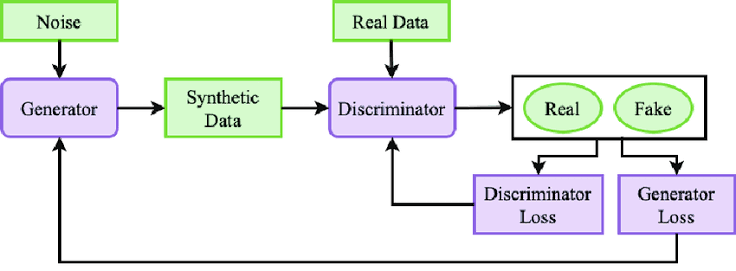
\includegraphics[width=1.0\textwidth]{intro_concepts/images/gan_architecture.png}
    \caption{Standard GAN architecture}
    \label{GAN_architecture}
\end{figure}

Moreover, as proved in \cite{background:gan}, for a fixed generator, the optimal discriminator can be derived analytically, obtaining the following expression:

\begin{equation}
D_G^*(x)
=
\frac{p_{data}(x)}
{p_{data}(x)+p_g(x)}.
\label{eq:optimal_discriminator}
\end{equation}

Where $p_g(x)$ is the distribution induced by the generator, equivalent to the distribution of the generated samples $G(z)$ when $z \sim p_z(z)$. 
Substituting this expression into the original minimax objective gives:

\begin{equation}
V(G,D_G^*)
=
- \log(4)
+
2 \cdot
JSD(p_{data}||p_g),
\label{eq:GAN_JS}
\end{equation}

where $JSD$ denotes the Jensen--Shannon divergence between the real and
generated distributions. Therefore, minimizing the GAN objective is equivalent to minimizing the
Jensen--Shannon divergence between the generated distribution and the true
data distribution, so when the generator is also optimal $p_g = p_{data}$ then the objective function reaches its minimum at $-\log(4)$.
Unfortunately, this remains a theoretical result 
since it is not possible, usually, to compute the optimal discriminator in practice,
and the training of GANs is often unstable and prone to issues such as mode collapse and vanishing gradients which will be discussed more in detail later on.\\


Despite the simplicity of the original formulation, GAN training suffers from
several fundamental difficulties.
The main issues include unstable optimization, vanishing gradients, mode
collapse, and sensitivity to hyperparameter choices.\\
These problems arise mainly because the discriminator and generator are
optimized simultaneously in a non-convex game.
Unlike classical optimization problems, where a unique minimum can often be
identified, GAN training seeks a Nash equilibrium between two competing
players.\\

Arjovsky and Bottou~\cite{background:gan_train_problems} demonstrated that the original GAN
objective can lead to severe optimization difficulties when the generated and
real distributions lie on low-dimensional manifolds.
In high-dimensional spaces, the supports of $p_{data}$ and $p_g$ may have
little or no overlap, causing the Jensen--Shannon divergence to become
constant.
When the discriminator becomes optimal too quickly, it can perfectly
distinguish real and generated samples. In this situation 
$D(G(z))\rightarrow 0$
and the gradient received by the generator becomes extremely small, providing little information for improving its distributional approximation capabilities.
This phenomenon is known as the \textit{vanishing gradient problem}.\\

Furthermore, GAN optimization may exhibit oscillatory behaviour rather than
convergence.
Mescheder et al.~\cite{background:gan_train_problems2} showed that simultaneous gradient-based
optimization does not necessarily converge to the desired Nash equilibrium,
even when the theoretical optimum exists.\\

These limitations become particularly relevant when GANs are applied to
financial time series. Unlike image datasets, financial observations are characterized by non-stationarity,
 regime changes, noisy stochastic dynamics and heavy tails distribution.
Therefore, instability in adversarial training may directly affect the quality
of generated financial scenarios and the reliability of downstream applications
such as risk estimation and derivative pricing.

Academic findings highlighted in \cite{background:gan_time_series} suggest that one of the principal failure modes of GANs 
arises when the generator converges to a parameter configuration that yields only a limited variety of outputs.
Existing research indicates that the occurrence of mode collapse is attributed to the establishment of a local 
equilibrium within the minimax optimization framework.
A further critical challenge involves the vanishing gradient problem,
which emerges when the discriminator becomes overly proficient,
causing the generator's gradients to approach zero and consequently impeding its learning process.\\


The original GAN framework learns the unconditional distribution
$p_{data}(x)$ and generates samples independently of any additional
information. However, many practical applications require the generation of
samples conditioned on external variables. In particular, in financial
forecasting the objective is not simply to generate realistic asset prices,
but rather to estimate the conditional distribution of future prices given
historical market information.\\
Conditional Generative Adversarial Networks (CGANs), introduced by Mirza and
Osindero~\cite{background:cgan}, extend the original GAN architecture by incorporating
additional information into both the generator and discriminator networks.
The conditioning variable can represent any relevant contextual information,
such as class labels, historical observations, market indicators, or previous
time-series values.\\
Let $c$ denote the conditioning variable. In the context of financial
forecasting, $c$ may represent the observed trajectory of an asset over a
historical window $c_t=(x_{t-k+1},x_{t-k+2},...,x_t)$ where $k$ denotes the length of the historical observation window.\\
The objective of a conditional generator is to learn the conditional
distribution $p(x|c)$ and generate samples that are consistent with the provided context $c$.\\

The generator receives both the latent noise vector $z$ and the conditioning
information $c$ while the discriminator evaluates whether a sample is consistent with the
conditioning information.
The conditional discriminator therefore does not only determine whether a
sample is realistic, but also whether it is compatible with the given
condition.
The CGAN objective function is given by:


\begin{equation}
    \label{eq:CGAN minimax}
    \min _G \max _D V(D, G)=\mathbb{E}_{\boldsymbol{x} \sim p_{\text {data }}(\boldsymbol{x})}[\log D(\boldsymbol{x} \mid \boldsymbol{c})]+\mathbb{E}_{\boldsymbol{z} \sim p_{\boldsymbol{z}}(\boldsymbol{z})}[\log (1-D(G(\boldsymbol{z} \mid \boldsymbol{c})))]
\end{equation}

A standard way for training GANs can be summarized by the following algorithm:

\begin{algorithm}[H]
\caption{Standard Conditional CGAN Training}
\label{alg: cgan}
\begin{algorithmic}[1]
\REQUIRE Initial discriminator parameters $\theta_D$, initial generator parameters $\theta_G$, condition matrix $C$, output data $X$.
\WHILE{$\theta_G$ has not converged}
    \STATE Sample real data $\{x^{(i)}\}_{i=1}^m \sim \mathbb{P}_{data}$ and context $\{c^{(i)}\}_{i=1}^m$.
    \STATE Sample latent noise $\{z^{(i)}\}_{i=1}^m \sim p_z$.
    \STATE $\tilde{x}^{(i)} \leftarrow G(z^{(i)}, c^{(i)})$ \COMMENT{Generate synthetic samples}
    
    \STATE \COMMENT{Update Discriminator: Maximize log(D(x)) + log(1-D(G(z)))}
    \STATE $L_{D} \leftarrow -\frac{1}{m} \sum_{i=1}^m \left[ \log D(x^{(i)}, c^{(i)}) + \log(1 - D(\tilde{x}^{(i)}, c  ^{(i)})) \right]$
    \STATE $\theta_D \leftarrow \theta_D - \alpha \nabla_{\theta_D} L_{D}$ \COMMENT{Gradient descent and backpropagation}
    
    \STATE Sample latent noise $\{z^{(i)}\}_{i=1}^m \sim p_z$.
    \STATE \COMMENT{Update Generator: Maximize log(D(G(z))) } 
    \STATE $L_{G} \leftarrow -\frac{1}{m} \sum_{i=1}^m \log D(G(z^{(i)}, c^{(i)}))$
    \STATE $\theta_G \leftarrow \theta_G - \alpha \nabla_{\theta_G} L_{G}$ \COMMENT{Gradient descent and backpropagation}
\ENDWHILE
\end{algorithmic}
\end{algorithm}


\section{Wasserstein GANs and other improvements}
The instability of the original GAN and (inherently the CGAN as well) formulation motivated the development of
alternative training objectives.
A major contribution was introduced by Arjovsky, Chintala and Bottou
through the Wasserstein GAN (WGAN) framework~\cite{background:wgan}.
The key idea behind WGAN is to replace the Jensen--Shannon divergence used in
the original GAN objective with the Wasserstein distance, also known as the
Earth Mover distance which measures the minimum cost required to transform one
probability distribution into another.

The transition from traditional divergence-based
Generative Adversarial Networks to those utilizing the Wasserstein metric 
represents a significant shift in the geometric treatment of probability 
measures within deep learning. 
The primal definition of the Wasserstein-1 distance 
for two probability distributions, $\mathbb{P}_r$ (real) and $\mathbb{P}_g$ (generated) is given 
by:
\begin{equation*}
    W(\mathbb{P}_r, \mathbb{P}_g) = \inf_{\pi \in \Pi(\mathbb{P}_r, \mathbb{P}_g)} \mathbb{E}_{(x, y) \sim \pi} [\|x - y\|]
\end{equation*}
where $\Pi(\mathbb{P}_r, \mathbb{P}_g)$ denotes the set of all joint distributions $\pi(x, y)$ with marginals $\mathbb{P}_r$ and $\mathbb{P}_g$.
While this formulation provides a physically intuitive measure of "work" required to transform one distribution into another, in fact this calculates the minimum "cost" of transporting mass to transform one distribution into the other.
It is computationally intractable in the context of neural networks because the infimum over the space of 
all possible transport plans $\pi$ cannot be efficiently optimized via backpropagation as suggested in \cite{background:wgan}.
Moreover, even if the two distributions are discretized through a binning strategy, an high computational cost is associated with the simulation of terminal values which define the empirical distribution and the following
discretization and evaluation of the Wasserstein distance.\\

To bridge this gap, CWGAN models rely on the \emph{Kantorovich-Rubinstein duality} \cite{intro:duality}, which transforms the constrained minimization over transport plans into a maximization over a set of 1-Lipschitz continuous functions.
The application of this duality is critical because it replaces the search for a transport plan with a search for a function $f$ (often called the Critic) that maximizes the difference between the expected values of the two distributions.\\


The main changes that characterize the CWGAN with respect to the CGAN are:
\begin{itemize}
    \item The loss function of a standard GAN is based on Jensen-Shannon divergence minimization while the CWGAN is based on the Wasserstein distance, which provides a more stable training process and mitigates issues such as mode collapse.
    \item The discriminator, which in Wasserstein GAN architecture is called critic, is designed to output real-valued scores instead of probabilities, allowing it to better capture the differences between real and generated data distributions.
    For this reason, the discriminator network does not use a sigmoid activation function in the output layer.
    \item The use of gradient penalty term in the loss function has the objective to enforce the Lipschitz constraint required for the Wasserstein distance computation.    
\end{itemize}

\begin{theorem}[Kantorovich duality]
\label{eq:kantarovich}
Let $(\mathcal{X}, \mu)$ and $(\mathcal{Y}, \nu)$ be two Polish probability spaces and let $c : \mathcal{X} \times \mathcal{Y} \to \mathbb{R} \cup \{+\infty\}$ be a lower semicontinuous cost function, such that
\begin{equation*}
    \forall(x,y) \in \mathcal{X} \times \mathcal{Y}, \quad c(x,y) \geq a(x) + b(y)
\end{equation*}
for some real-valued upper semicontinuous functions $a \in L^1(\mu)$ and $b \in L^1(\nu)$. Then
\begin{itemize}
    \item[(i)] There is duality:
\end{itemize}
\begin{align*}
    \min_{\pi \in \Pi(\mu, \nu)} & \int_{\mathcal{X} \times \mathcal{Y}} c(x, y) \, d\pi(x, y) \\
    &= \sup_{(\psi, \phi) \in C_b(\mathcal{X}) \times C_b(\mathcal{Y}); \,\, \phi-\psi \leq c} \left( \int_{\mathcal{Y}} \phi(y) \, d\nu(y) - \int_{\mathcal{X}} \psi(x) \, d\mu(x) \right) \\
    &= \sup_{(\psi, \phi) \in L^1(\mu) \times L^1(\nu); \,\, \phi-\psi \leq c} \left( \int_{\mathcal{Y}} \phi(y) \, d\nu(y) - \int_{\mathcal{X}} \psi(x) \, d\mu(x) \right) \\
    &= \sup_{\psi \in L^1(\mu)} \left( \int_{\mathcal{Y}} \psi^c(y) \, d\nu(y) - \int_{\mathcal{X}} \psi(x) \, d\mu(x) \right) \\
    &= \sup_{\phi \in L^1(\nu)} \left( \int_{\mathcal{Y}} \phi(y) \, d\nu(y) - \int_{\mathcal{X}} \phi^c(x) \, d\mu(x) \right),
\end{align*}
and in the above suprema one might as well impose that $\psi$ be $c$-convex and $\phi$ $c$-concave.
\end{theorem}

To formalize the components of the Kantorovich duality
within the context of Wasserstein GANs (WGANs), 
we define the underlying mathematical structures and their functional roles.
In this framework, the pairs $(\mathcal{X}, \mu)$ and $(\mathcal{Y}, \nu)$ 
represent Polish probability spaces, where in the specific case of generative modeling,
$\mu$ corresponds to the real data distribution $P_r$ and $\nu$ represents the model's 
generated distribution $P_g$. The cost function $c(x, y) \colon \mathcal{X} \times \mathcal{Y} \to \mathbb{R} \cup \{+\infty\}$ serves as the metric 
for the "work" required to transport a unit of mass from a point $x$ in the real domain to a point $y$ 
in the generated domain. The central object of the primal problem is the transport plan $\pi \in \Pi(\mu, \nu)$, 
which is a joint distribution whose marginals are constrained to $\mu$ and $\nu$. 
This plan describes the optimal allocation of mass across the product space.
Transitioning to the dual formulation introduces the dual potentials $\phi$ and $\psi$.
In the architecture of a WGAN, the potential $\phi$ (often denoted as $f$) is parameterized as the Critic network.
These functions assign scalar values to points in the manifold, effectively measuring the "potential energy" difference used to calculate the Wasserstein distance. Mathematically,
these potentials reside in $L^1(\mu)$, the space of functions that are integrable with respect 
to the measure $\mu$. A critical component for achieving the final loss function is the $c$-transform (or $c$-conjugate) of $\phi$, defined as:

\begin{equation}
    \phi^c(x) = \inf_{y \in \mathcal{Y}} [c(x, y) - \phi(y)]
\end{equation}

This transform identifies the optimal "mate"
function that satisfies the feasibility constraint
$\phi(y) - \psi(x) \leq c(x, y)$. When the cost function $c(x, y)$
is chosen as the $L_1$ distance $\|x - y\|$, the $c$-transform forces 
$\phi$ to satisfy a Lipschitz continuity constraint. 
This transformation is what allows the WGAN to replace the intractable search over all transport plans $\pi$ with a simpler maximization over $1$-Lipschitz functions, 
providing the stable gradients necessary for training deep generative models.

So finally, the Kantorovich-Rubinstein duality can be expressed in the specific case of the Wasserstein-1 distance, given
$P_r$ and $P_g$ two probability distributions defined on a compact metric space $\mathcal{X}$ and where
the supremum is taken over all $1$-Lipschitz continuous functions $f: \mathcal{X} \to \mathbb{R}$, such that for all $x, y \in \mathcal{X}:   |f(x) - f(y)| \leq \|x - y\|$, then:
\begin{equation}
    \label{eq: emd_dual}
    W(P_r, P_g) = \sup_{\|f\|_L \leq 1} \left( \mathbb{E}_{x \sim P_r}[f(x)] - \mathbb{E}_{x \sim P_g}[f(x)] \right)
\end{equation}


In this duality, the "discriminator" is redefined as a "critic" ($D$), whose task is not to classify
inputs as real or fake, but to act as the optimal function $f$ that maximizes the distance between the 
expected scores of the real and synthetic distributions.
In the following thesis, $f$ is parametrized by using a neural network $f_w$ with weights $w$ restricted to a compact space $\mathcal{W}$ to enforce the Lipschitz constraint.
Substituting the generator output $G(z)$ for samples from $P_g$, the optimization objective function for the Wasserstein GAN is obtained.
The minimax objective function is the following:
\begin{equation}
    \label{eq:wgan_objective_function}
    L(G, f_w) = \min_G \max_{w \in \mathcal{W}} \mathbb{E}_{x \sim P_r}[f_w(x)] - \mathbb{E}_{z \sim p(z)}[f_w(G(z))]
\end{equation}
By enforcing $\|f_w\|_L \leq K$ (where $K$ is a constant, typically through weight clipping or gradient penalty), the Critic provides a linear, non-saturating gradient to the Generator, ensuring stable training even when the Generator is far from the target distribution.

In a Conditional GAN (CGAN), this distance is 
extended to account for auxiliary information $c$ (such as past history, drift, or volatility in 
time-series). So in the conditional setting, 
mathematically, the EMD is calculated over the pairs $(x, c)$, where $c$ is the history and $x$ is the generated output.
The real pair $(x_{i, real}, c_i)$ and fake pair $(G(z_i, c_i), c_i)$ are produced. The "Earth mass" is not being moved on a 1D line but instead it is being moved in a higher-dimensional space where one axis is the context and the other is the generated output. 
The distance is only minimized when the generator produces the correct $x$ for that specific $c$.

The objective becomes the minimization of the Wasserstein distance between the 
conditional distributions $\mathbb{P}_r(x|c)$ and $\mathbb{P}_g(x|c)$. 
By conditioning both the generator $G(z, c)$ and the critic $D(x, c)$ on the same context $c$,
the critic learns a "score surface" that is specific to the underlying stochastic process defined by $c$.

The use of the critic's output to compute the loss is mathematically 
justified because, under the 1-Lipschitz constraint, 
the difference between the average scores of the real batch and 
the fake batch directly approximates the Wasserstein distance as demonstrated in \cite{background:wgan}.
This is a superior training signal compared to Jensen-Shannon divergence because
$W(\mathbb{P}_r, \mathbb{P}_g)$ is
continuous and differentiable even when the supports of the two
distributions are disjoint, a common occurrence in the early stages of training.
Consequently, the generator receives stable, non-vanishing gradients that indicate 
not just if the generated sample is wrong,
but how far it must move in the feature space to align with the real
data manifold. 
To enforce the Lipschitz constraint required by the duality, modern implementations utilize a Gradient Penalty (GP),
which regularizes the norm of the critic's gradient with respect to its input toward unity, ensuring the function remains 
within the space of 1-Lipschitz functions $\mathcal{D}$.

\begin{algorithm}[H]
\caption{Conditional Wasserstein GAN with Gradient Penalty (CWGAN-GP)}
\label{alg:cwgan_gp}
\begin{algorithmic}[1]
\REQUIRE The gradient penalty coefficient $\lambda$, the number of critic iterations per generator iteration $n_{critic}$, the batch size $m$, Adam hyperparameters $\alpha, \beta_1, \beta_2$.
\REQUIRE Initial critic parameters $\theta_D$, initial generator parameters $\theta_G$.
\WHILE{$\theta_G$ has not converged}
    \FOR{$t = 1$ \TO $n_{critic}$}
        \STATE Sample real data $\{x^{(i)}\}_{i=1}^m \sim \mathbb{P}_r$ and context $\{c^{(i)}\}_{i=1}^m$.
        \STATE Sample latent noise $\{z^{(i)}\}_{i=1}^m \sim \mathbb{P}_z$.
        \STATE $\tilde{x}^{(i)} \leftarrow G(z^{(i)}, c ^{(i)})$ \COMMENT{Generate synthetic samples}
        \STATE $\epsilon \sim U[0, 1]$ \COMMENT{Random number for interpolation}
        \STATE $\hat{x}^{(i)} \leftarrow \epsilon x^{(i)} + (1 - \epsilon) \tilde{x}^{(i)}$ \COMMENT{Interpolated samples} 
        \STATE $L_{D} \leftarrow \frac{1}{m} \sum_{i=1}^m D(\tilde{x}^{(i)}, c^{(i)}) - \frac{1}{m} \sum_{i=1}^m D(x^{(i)}, c^{(i)}) + \lambda \mathbb{E}_{\hat{x}, c} [(\|\nabla_{\hat{x}} D(\hat{x}, c)\|_2 - 1)^2]$  
        \STATE $\theta_D \leftarrow \text{Adam}(\nabla_{\theta_D} L_{D}, \theta_D, \alpha, \beta_1, \beta_2)$
    \ENDFOR
    
    \STATE Sample latent noise $\{z^{(i)}\}_{i=1}^m \sim \mathbb{P}_z$.
    \STATE $L_{G} \leftarrow -\frac{1}{m} \sum_{i=1}^m D(G(z^{(i)}, c^{(i)}))$
    \STATE $\theta_G \leftarrow \text{Adam}(\nabla_{\theta_G} L_{G}, \theta_G, \alpha, \beta_1, \beta_2)$
\ENDWHILE
\end{algorithmic}
\end{algorithm}

An import part of the training procedure is the gradient penalty calculation, which is described in Algorithm \ref{alg:gradient_penalty}.
By sampling $\epsilon$ and creating $\hat{x}$, the Lipschitz constraint is enforced specifically on the straight lines between the real and fake data manifolds.

\begin{algorithm}[H]
\caption{Gradient Penalty Calculation for CWGAN-GP}
\label{alg:gradient_penalty}
\begin{algorithmic}[1]
\REQUIRE Real samples $x$, generated samples $\tilde{x}$, conditioning context $c$, critic network $D$.
\STATE $m \leftarrow \text{batch size}$
\STATE Sample $\epsilon \sim U[0, 1]^m$ \COMMENT{Uniform random interpolation weights}
\STATE $\hat{x} \leftarrow \epsilon x + (1 - \epsilon) \tilde{x}$ \COMMENT{Compute interpolated samples}
\STATE Enable gradient tracking for $\hat{x}$
\STATE $\hat{S} \leftarrow D(\hat{x}, c)$ \COMMENT{Evaluate critic on interpolates}
\STATE $\nabla_{\hat{x}} D \leftarrow \nabla_{\hat{x}} \hat{S}$ \COMMENT{Compute gradients of scores w.r.t. interpolates}
\STATE $L_2 \text{-norm} \leftarrow \|\nabla_{\hat{x}} D(\hat{x}, c)\|_2$ \COMMENT{Calculate norm across feature dimensions}
\STATE $GP \leftarrow \frac{1}{m} \sum (L_2 \text{-norm} - 1)^2$ \COMMENT{Compute mean squared error from unity}
\RETURN $GP$
\end{algorithmic}
\end{algorithm}

So the final objective function for the Conditional Wasserstein GAN with gradient penalty (CWGAN-GP) becomes:

\begin{equation}
    \begin{aligned}
        \min _G \max _D V(D, G) = & \mathbb{E}_{\boldsymbol{x} \sim p_{\text {d}}}[D(\boldsymbol{x} \mid \boldsymbol{c})] - \mathbb{E}_{\boldsymbol{z} \sim p_{\boldsymbol{z}}}[D(G(\boldsymbol{z} \mid \boldsymbol{c}))] + \lambda GP
    \end{aligned}
\end{equation}
where $\lambda$ is a hyperparameter that controls the strength of the penalty and it is usually set to $10$ as suggested in \cite{background2:gp_wgan}.\\
An additional advantage of using the Wasserstein distance is that it provides a meaningful measure of the distance between the real and generated data distributions, which allows for the implementation of an early stopping technique which
improve the training efficiency.\\

When the generated distribution and real distribution are far apart, the
Jensen--Shannon divergence often becomes constant.
Consequently, the discriminator saturates and the generator receives
vanishing gradients. Conversely, the Wasserstein distance changes continuously as the generated
distribution moves toward the target distribution.
Therefore, even when the two distributions have limited overlap, the critic
provides meaningful gradient information.\\

Other tentatives to improve the stability of GAN training. One of the most successful techniques are the spectral normalization and feature matching.
Miyato et al.~\cite{background:spectral_norm} proposed Spectral Normalization as a method to
control the Lipschitz constant of neural networks. The weight matrix of each discriminator layer is normalized according to its
spectral norm: $\bar{W}=\frac{W}{\sigma(W)}$
where $\sigma(W)$ represents the largest singular value of $W$.
Spectral normalization constrains discriminator updates and improves
stability without requiring additional gradient penalties.
It has become one of the most effective stabilization techniques for modern
GAN architectures.\\

Salimans et al.~\cite{background:feature_matching} introduced feature matching as a method to
reduce mode collapse. Instead of directly maximizing discriminator classification error, the
generator minimizes the difference between statistics of intermediate
discriminator features:

\begin{equation*}
L_G
=
\left|
\mathbb{E}_{x\sim p_{data}}D(x)
-
\mathbb{E}_{z\sim p_z}D(G(z))
\right|^2 .
\end{equation*}

This encourages the generator to reproduce multiple modes of the target
distribution rather than exploiting weaknesses of the discriminator.


\section{GANs for Time Series}
The architectures reviewed so far in this chapter, 
the original GAN, its conditional extension, and the variance-reduction/stabilization techniques, were developed 
primarily with static, i.i.d. data, most prominently images, in mind. 
Extending the adversarial framework to \emph{sequential} data introduces a distinct
set of architectural requirements: 
the generator and discriminator must be able to represent
temporal dependence, like autocorrelation, rather than merely a single, 
unconditional multivariate distribution, and, for variable-length or streaming applications, 
must do so with a fixed-size internal state rather than a fixed-size input/output tensor. 
This section reviews the principal families of sequential GAN architectures, 
culminating in the financial-time-series-specific 
proposals that directly motivate the modelling choices made later in this thesis.\\

The most direct way to extend a GAN to sequential data is to replace the feed-forward generator and discriminator networks of the original architecture with recurrent networks (LSTMs or GRUs) that process a sequence one step at a time,
propagating a hidden state $\mathbf{h}_\tau$ forward across the sequence index $\tau$. 
A generic recurrent generator produces a sequence $\hat{\mathbf{x}}_{1:H} = (\hat x_1, \dots, \hat x_H)$ autoregressively,
\begin{equation*}
\hat x_\tau = g_\theta\left(\mathbf{h}_{\tau-1}, z_\tau\right), \qquad \mathbf{h}_\tau = f_\theta\left(\mathbf{h}_{\tau-1}, \hat x_\tau, z_\tau\right), \qquad \tau = 1,\dots,H,
\end{equation*}

\cite{background:rcgan} propose the Recurrent Conditional GAN (RCGAN), developed originally for the generation of realistic multivariate medical time series. RCGAN uses an RNN (LSTM) for both generator and discriminator, with the generator receiving \emph{independent} noise draws at every time step rather than a single noise vector at initialization,
\begin{equation*}
\hat x_\tau = G_\theta\left(\mathbf{h}_{\tau-1}, z_\tau\right), \qquad z_\tau \stackrel{\text{iid}}{\sim} \mathcal{N}(0, I),
\end{equation*}
a design choice the authors show empirically increases sample diversity relative to single-noise-vector variants, directly counteracting the temporal mode-collapse tendency whereby a generator conditioned on a single static noise draw tends to produce sequences that are smooth, low-entropy interpolations rather than genuinely stochastic paths. The discriminator likewise processes the full sequence recurrently and is trained with the standard (or, in later variants, Wasserstein) adversarial loss applied either to the final hidden state or averaged across per-step outputs. RCGAN additionally supports conditioning on auxiliary static or time-varying labels.\\

Also \cite{background:timegan} propose a novel architecture for time series generation that addresses a specific shortcoming of purely adversarial recurrent GANs: 
the adversarial loss alone provides no explicit incentive for the 
generator to preserve the \emph{stepwise conditional} dynamics 
of the training data (i.e. the transition structure $p(x_\tau \mid x_{1:\tau-1})$), since the discriminator, 
in its simplest form, only ever evaluates entire generated sequences 
(or fixed-length windows) against real ones in aggregate, without an explicit term that penalizes mismatches in 
the one-step-ahead transition law. TimeGAN addresses this by combining the adversarial objective with a 
\emph{supervised} autoregressive loss, and by decoupling the 
space in which the generator operates from the original data space via a 
learned embedding.\\

The proposed architectures for time series proposed so far are designed for the generation of realistic sequences, but do not directly address the problem of \emph{forecasting}, 
where the goal is to estimate the conditional distribution of future values given a history. One of the most influential architectures in this space is ForGAN \cite{background:forgan}, 
which combines the conditional adversarial framework with a recurrent conditioning network.

\section{Probabilistic Forecasting using GANs}
The overwhelming majority of forecasting models developed in the quantitative finance and machine learning literature are trained to minimize a pointwise loss function, typically the mean squared error (MSE) or the mean absolute error (MAE), between a predicted scalar or vector and an observed realization. Formally, given a conditioning history $\mathbf{x}_{1:t} = (x_1, \dots, x_t)$ of a stochastic process, a point forecaster learns a deterministic mapping
\begin{equation*}
\hat{x}_{t+1} = f_\theta(\mathbf{x}_{1:t}), \qquad \theta^\star = \arg\min_\theta \; \mathbb{E}\left[ \ell\left(x_{t+1}, f_\theta(\mathbf{x}_{1:t})\right) \right],
\end{equation*}
where $\ell(\cdot,\cdot)$ is typically the squared error $\ell(x,\hat x) = (x-\hat x)^2$.
When the underlying data-generating process is stochastic, as is the case for essentially every financial time series, since asset prices, volatilities, and interest rates evolve under genuine aleatoric uncertainty, a point forecast conveys only the conditional mean (or, depending on the loss, the conditional median) of the future state, and discards all information about the shape, skewness, and tail behaviour of the conditional distribution.
This is a critical shortcoming for financial applications, where risk management, derivatives pricing, and portfolio construction depend fundamentally on the full conditional law of future returns rather than on a single expected value.\\

The correct object of interest is therefore the conditional predictive distribution
\begin{equation}
p\left(x_{t+1} \mid \mathbf{x}_{1:t}\right),
\end{equation}
or, in the multi-step-ahead case relevant to path-dependent risk metrics, the joint conditional distribution
\begin{equation}
p\left(x_{t+1}, x_{t+2}, \dots, x_{t+H} \mid \mathbf{x}_{1:t}\right)
\end{equation}
over a forecast horizon $H$. 
Estimating this object is the task of \emph{probabilistic forecasting} \cite{background:probabilistic_forecasting}. 
Classical approaches to probabilistic forecasting in econometrics rely on explicit parametric assumptions, for example, GARCH-family models coupled with a Gaussian or Student-$t$ innovation distribution,
or the Heston stochastic volatility model itself, 
which specifies a closed-form (up to Fourier inversion) 
characteristic function for the conditional log-price distribution. 
These approaches are interpretable and computationally tractable, 
but their accuracy is contingent on the correctness of the parametric assumption; 
misspecification of the innovation distribution or of the volatility dynamics propagates directly into biased risk estimates.\\

Generative Adversarial Networks 
offer an attractive alternative precisely
because they are implicit generative models
where the generator $G(\mathbf{c}, \mathbf{z})$, conditioned on a history $\mathbf{c} = \mathbf{x}_{1:t}$ 
and driven by an exogenous noise vector $\mathbf{z} \sim p_z$, is trained so that its induced output distribution approximates $p(x_{t+1} \mid \mathbf{x}_{1:t})$
without any parametric assumption on the shape of that distribution. 
Repeated sampling of $\mathbf{z}$ for a fixed conditioning history $\mathbf{c}$ produces an empirical ensemble of trajectories, from which arbitrary functionals of the predictive distribution, quantiles, moments, tail probabilities and so on,
can be estimated by Monte Carlo. This is the conceptual bridge between adversarial generative modelling and probabilistic time series forecasting,
and it is the foundation of the ForGAN architecture discussed below.\\

ForGAN, introduced by \cite{background:forgan},
is a conditional GAN architecture designed
explicitly for one-step-ahead probabilistic
forecasting of univariate time series. 
It combines the conditional adversarial training framework
with a recurrent conditioning network, so that the generator 
can encode an arbitrarily long history into a fixed-dimensional context vector 
before producing a sample of the next-step distribution.\\

The ForGAN's architecture is based on a generator and a discriminator, both utilizing Recurrent Neural Network (RNN) layers, specifically LSTM or GRU variants, in order to process sequential data.\\
The generator's objective is to forecast a future next value $x_{t+h}$ by transforming the noise vector $z$, 
conditioned on the historical window $c$.\\
The probability distribution of $x_{t+h}$ is modeled as $P(x_{t+h}|c)$ and obtained by running the generator multiple times with different noise inputs and same condition window $c$.\\
Structurally, the generator processes the condition window $c$ through an RNN layer to construct a "condition representation" whose size is given by hidden state size.
This representation is subsequently concatenated with the noise vector $z$.
The combined feature vector is then passed through two dense layers, culminating in a single scalar output representing the predicted $x_{t+h}$.\\
On the other hand, the discriminator has the role to inspect the validity of a given value $x_{t+h}$ in the context of the history $c$.
Unlike standard discriminators that might process inputs separately, the ForGAN discriminator takes the candidate $x_{t+h}$, which is sourced either from the ground truth dataset or the generator, and concatenates it to the end of the condition window $c$, forming an extended sequence $\{x_{0},...,x_{t+h}\}$.
This extended sequence is fed into an RNN layer, followed by a dense layer that outputs a validity score, determining whether the sequence is real or generated.
So the innovation is given by the presence of a conditioner which is implemented as a recurrent neural network that processes the conditioning window $\mathbf{c} = (x_{t-\ell+1}, \dots, x_t)$ of length $\ell$ and returns the terminal hidden state as a fixed-length embedding,
\begin{equation}
C_\phi(\mathbf{c}) = \mathrm{RNN}_\phi(x_{t-\ell+1}, \dots, x_t) \in \mathbb{R}^{d_c}.
\end{equation}\\

\begin{figure}[H]
    \centering
    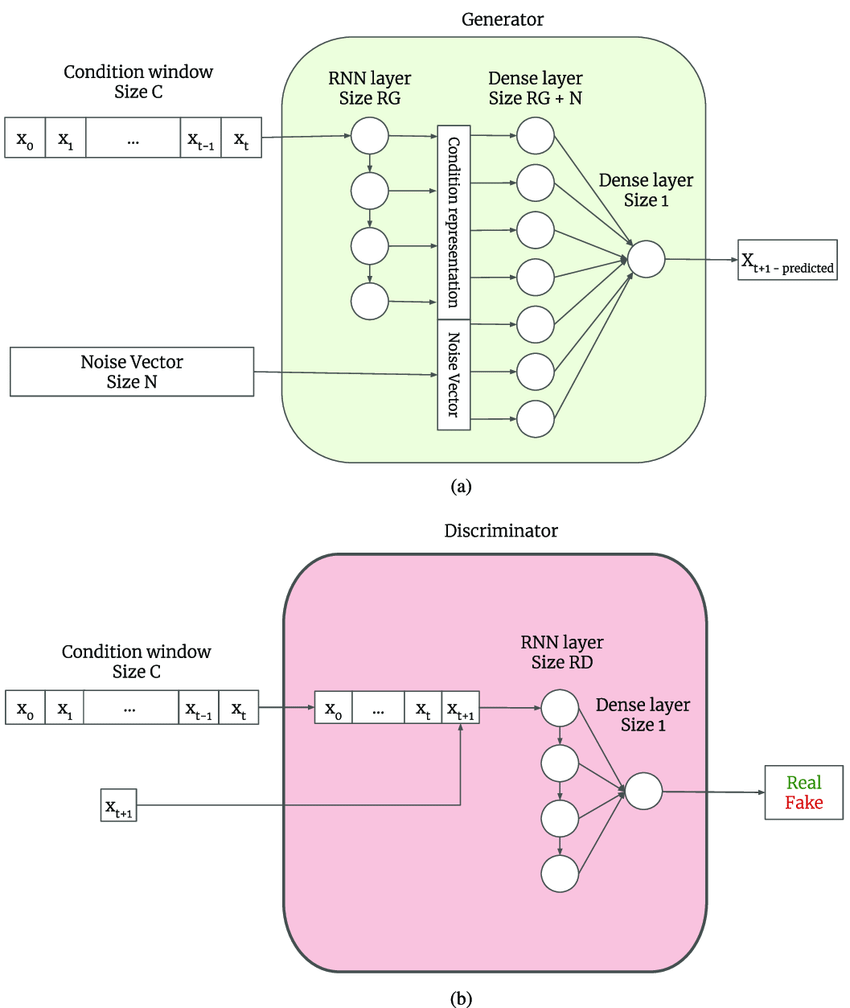
\includegraphics[width=1.0\textwidth]{Introduction/images/forgan_rnn.png}
    \caption{ForGAN building blocks}
    \label{img:forgan_rnn}
\end{figure}

\begin{figure}[H]
    \centering
    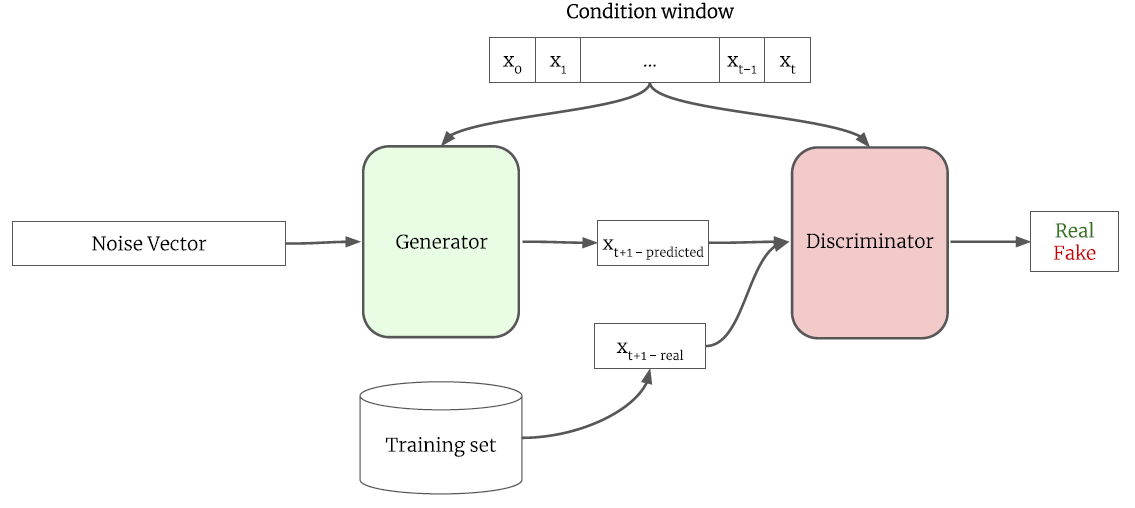
\includegraphics[width=1.0\textwidth]{Introduction/images/forgan.png}
    \caption{ForGAN architecture}
    \label{img:forgan}
\end{figure}

The model is trained with the standard conditional minimax objective adapted to the time series conditioning structure. In fact, as proposed in \cite{background:forgan}, the objective is to minimize the Jensen-Shannon divergence between the real and generated data as seen before \ref{eq:CGAN minimax}.
Because the original ForGAN objective inherits the training pathologies
of the vanilla GAN, like vanishing gradients when the discriminator saturates,
and susceptibility to mode collapse (see Section~\ref{sec:limitations-gans}), 
a natural extension replaces the Jensen--Shannon-based minimax loss with the Wasserstein critic loss \ref{eq:wgan_objective_function}.
In this last case the model can be referenced as ForWGAN which represent a novel 
approach to increase the performance of the standard ForGAN.\\

While ForGAN 
was shown to perform strongly on the sensory
and synthetic benchmarks
for which it was originally developed, \cite{forgan:fin_gan} directly investigate 
its behaviour on financial return data, 
and show that a ForGAN trained with its original, 
generic binary-cross-entropy (BCE) adversarial loss is \emph{systematically outperformed},
on economically meaningful metrics, by both classical econometric baselines (ARIMA)
and by a variant of the same ForGAN architecture trained with a purpose-built, 
economics-driven loss function, the proposed Fin-GAN model.
This result is important for the present thesis because it demonstrates 
that the limitations catalogued in Section~\ref{sec:limitations-gans} 
are not merely a theoretical curiosity: 
they have a directly measurable, negative impact on downstream financial performance,
specifically in the ForGAN architecture that the SRForGAN model developed in this thesis builds upon.\\
The core diagnosis in \cite{forgan:fin_gan} 
is a form of \emph{objective misalignment} between what the ForGAN 
adversarial loss actually optimizes and what a 
financial forecasting application actually requires. 
In the Fin-GAN paper, the authors solve the inherent misalignment of the BCE-trained ForGAN by replacing the generic adversarial loss with a composite loss function that explicitly encodes 
the financial decision-making objectives of interest, 
including mean-squared error, sign accuracy, profit-and-loss, and risk-adjusted return. 
So, they worked on the loss function to make it more aligned with the financial forecasting task, 
rather than on the architecture itself. It is indeed, the same approach that is pursued in this thesis.\\


The Fin-GAN critique of BCE-trained ForGAN is,
in an important sense, structurally analogous to the motivation 
for the scoring-rule-based training paradigm underlying the SRForGAN architecture developed in this thesis.
Both approaches share the diagnosis that the original ForGAN training objective,
precisely because it is a generic adversarial divergence with no reference 
to the specific quantity the downstream application 
cares about, is an unreliable foundation for financial forecasting,
and both approaches respond by replacing that generic objective with one explicitly aligned 
to a well-defined target: 
in Fin-GAN's case, an economics-driven, 
decision-rule-specific composite loss 
(MSE, sign accuracy, PnL, and risk-adjusted-return terms); 
in the case of this thesis, a strictly proper scoring rule whose global minimizer is, 
by construction, the true conditional \emph{distribution} itself, 
rather than a decision-rule-specific functional of it.

\section{Scoring Rules and ForGAN advances}
The paradigm formalized by \cite{background:scoring_rules} 
is to jointly assess calibration and 
sharpness through \emph{proper scoring rules}: 
functionals $S(\hat P, x)$ of a predictive distribution $\hat P$ 
and a realized outcome $x$ such that the expected score 
is uniquely minimized when the forecaster 
reports the true conditional distribution,

\begin{equation}
\mathbb{E}_{x \sim P}\left[ S(P, x) \right] \le \mathbb{E}_{x \sim P}\left[ S(\hat P, x) \right] \qquad \text{for all } \hat P,
\end{equation}
with equality if and only if $\hat P = P$, a property known as strict propriety.
Proper scoring rules are the natural loss functions
for training and evaluating GAN-based probabilistic forecasters,
precisely because they can be estimated consistently
from samples, that is, without requiring an explicit likelihood,
which aligns with the implicit, 
sampling-based nature of the GAN generator.\\

The two proper scoring rules most relevant to this literature, and to the scoring-rule-based training paradigm are the Continuous Ranked Probability Score (CRPS) and the Energy Score.
For a univariate predictive CDF $\hat F$ and a scalar outcome $x$,
\begin{equation}
\mathrm{CRPS}(\hat F, x) = \int_{-\infty}^{\infty} \left( \hat F(y) - \mathbf{1}_{y \ge x} \right)^2 \, dy,
\end{equation}
which admits the equivalent, sample-based (kernel) representation in terms of two independent draws $X, X' \sim \hat F$,
\begin{equation}
\mathrm{CRPS}(\hat F, x) = \mathbb{E}\left| X - x \right| - \tfrac{1}{2}\, \mathbb{E}\left| X - X' \right|.
\end{equation}
This representation is directly usable as a training loss for a GAN generator: given $N$ samples $\{\hat x^{(i)}\}_{i=1}^N$ drawn from $G([\mathbf{c},\mathbf{z}^{(i)}])$, an unbiased estimator of the CRPS is
\begin{equation}
\widehat{\mathrm{CRPS}} = \frac{1}{N} \sum_{i=1}^{N} \left| \hat x^{(i)} - x_{t+1} \right| - \frac{1}{2 N (N-1)} \sum_{i=1}^{N} \sum_{j \neq i} \left| \hat x^{(i)} - \hat x^{(j)} \right|,
\end{equation}

The natural multivariate generalization of the CRPS, applicable when the forecast target is a vector $\mathbf{x} \in \mathbb{R}^d$ (e.g. a full multi-step forecast path, or a vector of Heston state variables), is the Energy Score of order $\beta \in (0,2)$:
\begin{equation}
\mathrm{ES}_\beta(\hat P, \mathbf{x}) = \mathbb{E}\left\| \mathbf{X} - \mathbf{x} \right\|_d^\beta - \tfrac{1}{2}\, \mathbb{E}\left\| \mathbf{X} - \mathbf{X}' \right\|_d^\beta, \qquad \mathbf{X}, \mathbf{X}' \stackrel{\text{iid}}{\sim} \hat P,
\end{equation}
which reduces to (twice) the CRPS when $d=1$ and $\beta=1$. As with the CRPS, the Energy Score is strictly proper for $\beta \in (0,2)$, and its sample estimator
\begin{equation}
\widehat{\mathrm{ES}}_\beta = \frac{1}{N}\sum_{i=1}^N \left\| \hat{\mathbf{x}}^{(i)} - \mathbf{x} \right\|_2^\beta - \frac{1}{2N(N-1)} \sum_{i=1}^N\sum_{j\ne i} \left\| \hat{\mathbf{x}}^{(i)} - \hat{\mathbf{x}}^{(j)} \right\|_2^\beta
\end{equation}

The Energy Score therefore plays a role directly analogous to the minimax value function $V(D,G)$ of the original GAN, but with the crucial advantage that it is a proper scoring rule with a known, well-behaved minimizer, removing the discriminator-induced gradient pathologies discussed in Section~\ref{sec:limitations-gans} at the cost of a bias--variance trade-off governed by the ensemble size $N$ (the estimator above is unbiased for the population Energy Score, but its variance decreases only at rate $O(1/N)$, so small ensembles yield noisy gradients.


\section{Applications in Quantitative Finance}
 
The appeal of adversarially or scoring-rule
trained generative models in quantitative 
finance stems from a structural feature 
shared by nearly every downstream task in the field: 
risk management, derivative pricing, and portfolio 
optimization all reduce, at some level, 
to computing an expectation (or a quantile, or a full distribution) 
of a functional of future asset paths. 
Classical Monte Carlo methods evaluate 
such expectations by simulating paths 
from an explicit, calibrated stochastic model 
(e.g. Heston, SABR, or a local-volatility model); 
GAN-based methods replace 
this explicit simulator with a 
learned, data-driven generator, 
potentially side-stepping model 
misspecification at the cost of 
requiring large amounts of 
representative historical data and 
forfeiting the interpretability of a closed-form model.\\

Distribution-valued
forecasting has a growing dedicated literature in finance.
\cite{background:quantile_regression} use a deep quantile-regression
network to forecast Value-at-Risk directly, 
reporting significant accuracy gains over linear quantile regression. 
A recent study \cite{background:applications} 
trains CNN and LSTM networks to output the parameters 
of skewed-$t$ predictive distributions, 
evaluating them with CRPS and PIT diagnostics 
and showing they are competitive with GARCH for 
VaR estimation. 
\cite{background:applications2} combine deep quantile regression with GAN-based scenario generation specifically to estimate VaR and Expected Shortfall jointly, explicitly motivating GAN-generated tail scenarios as a remedy for the difficulty classical models have capturing stressed regimes.\\

On the pricing side, generative and simulation-based deep models have been applied to option-market 
simulation and hedging, 
notably \cite{background:applications3}'s Deep Hedging framework and 
 Quant GAN for scenario generation. 
Also the work of \cite{background:applications4}, Tail-GAN, modify the adversarial objective itself to 
target VaR/ES elicitability directly, 
reflecting the same insight, 
that generic distributional losses under-serve the tail, 
that motivates using a proper scoring rule rather than a raw adversarial loss in SRForGAN. 
These works establish both the demand for, and the 
empirical viability of, GAN and neural-network-based 
probabilistic forecasters as inputs to standard risk and 
pricing pipelines, and SRForGAN can be positioned within 
this literature representing a suitable GAN-based architecture
capable of capturing the full conditional distribution of financial processes,
representing a valid alternative to parametric models and other generative architectures.




\section{Limitations of GANs}
\label{sec:limitations-gans}
Despite their theoretical appeal as flexible, likelihood-free generative models, GANs are notoriously difficult to train in practice, and the literature documenting and diagnosing their failure modes is nearly as extensive as the literature proposing new architectures. This section reviews the principal sources of instability, with particular attention to the manifestations that are most consequential for financial time-series applications.\\

The original GAN formulation establishes tha, in the nonparametric limit, that is when both $G$ and $D$ have unlimited capacity and are optimized exactly, alternately, to their respective optima at each step,
the minimax game converges to a unique Nash equilibrium at which $p_g = p_{\mathrm{data}}$. This guarantee, however, does not extend to the practically relevant setting in which $G$ and $D$ 
are finite-capacity neural networks trained by simultaneous or alternating stochastic gradient descent. 
In this setting, the minimax objective \ref{eq:GAN minimax}
defines a non-convex, two-player game,
for which simultaneous gradient descent is not guaranteed to converge even locally,
let alone to the desired Nash equilibrium. 
The resulting optimization landscape is known to exhibit oscillatory, non-convergent trajectories even on simple, low-dimensional toy problems,
where the generator and discriminator can enter a persistent limit cycle rather than converging to the equilibrium.\\

One of the most widely documented failure modes is \emph{mode collapse}, 
refers to the failure mode in which the generator $G$ learns to produce outputs concentrated on a small subset of the modes
(or, in the extreme case, a single point or a very low-dimensional manifold) of the true data distribution
$p_{\mathrm{data}}$,
rather than covering its full support.
The phenomenon arises, as discussed in \cite{background:mode_collapse}, because the minimax objective, when optimized via alternating gradient steps
rather than the idealized best-response dynamic assumed in the original convergence proof,
provides no direct incentive for the generator to maintain output diversity:
if a subset of the noise space $\mathcal{Z}$ maps to outputs that reliably fool the current discriminator,
gradient descent on parameters of $G$ has no mechanism to \emph{penalize} 
the generator for ignoring the remainder of $\mathcal{Z}$, since the objective is evaluated only in expectation over $\mathbf{z}$ and contains no explicit diversity or entropy term.\\
Actually, gradient descent effectively optimizes the cases in which the generator 
need only to find, for each fixed discriminator, \emph{some} output that fools it, rather than a full distribution that matches $p_{\mathrm{data}}$
under every possible discriminator. 
\cite{background:wgan} further connect mode collapse to a distributional-support argument:
when $p_{\mathrm{data}}$ and $p_g$ have disjoint or low-dimensional-overlapping supports
(a generic situation when both are supported on low-dimensional manifolds embedded in a high-dimensional ambient space, as is typically the case for both images and, arguably, financial processes),
the Jensen--Shannon divergence between them is \emph{constant} (equal to $\log 2$)
and its gradient with respect to the generator's parameters is zero almost everywhere, 
providing no useful training signal and creating an optimization landscape in which the generator can become ``stuck'' 
having covered only a subset of the target modes, 
with no local gradient information indicating the direction of the missing modes.\\
In the context of probabilistic financial forecasting, 
mode collapse manifests specifically as \emph{underdispersion}: 
a generator conditioned on a given history $\mathbf{x}_{1:t}$ 
collapses across noise draws $\mathbf{z}$ 
to a narrow cluster of outputs, so that the induced 
predictive distribution $\hat p_G(x_{t+1} \mid \mathbf{x}_{1:t})$ 
has substantially smaller variance than the true conditional distribution.\\

A second, related instability is the \emph{gradient vanishing} that arises from gradient saturation at the discriminator.
Recall the original generator loss $\mathbb{E}_{\mathbf z}[\log(1 - D(G(\mathbf z)))]$:
when the discriminator is properly trained, 
it rapidly learns to assign $D(x) \approx 1$
for real samples and $D(G(\mathbf z)) \approx 0$ 
for generated samples that are not yet realistic. 
In this regime,
\begin{equation}
\frac{\partial}{\partial \theta} \, \mathbb{E}_{\mathbf z}\left[ \log\left(1 - D_\psi(G_\theta(\mathbf z))\right) \right] \; \longrightarrow \; 0,
\end{equation}
with $\theta$ the discriminator parameters and $\phi$ the generator parameters. This happens because
the function $\log(1-y)$ has near-zero slope as $y \to 0$, 
so that precisely when the generator is performing poorly and most needs a strong corrective gradient,
the gradient it receives vanishes. 
\cite{background:gan} proposed the standard workaround, training the generator to instead maximize $\mathbb{E}_{\mathbf z}[\log D_\psi(G_\theta(\mathbf z))]$, which restores a non-vanishing gradient in the early-training, 
poorly-performing regime, but at the cost of abandoning the interpretation of the generator's objective 
as the minimization of a well-defined statistical divergence between $p_g$ and $p_{\mathrm{data}}$,
and reintroducing exactly the mode-seeking, 
diversity-agnostic behaviour discussed above. 
\cite{background:wgan} show more generally that, 
whenever the discriminator is allowed to approach optimality 
(which is precisely what is needed for it to provide an accurate estimate of any $f$-divergence, including the Jensen--Shannon divergence underlying the original GAN), 
the generator's gradient with respect to the Jensen--Shannon-based objective vanishes in the limit, 
establishing vanishing gradients not as an incidental implementation 
artifact but as a structural property of divergence-minimizing GAN objectives whenever $p_g$ and $p_{\mathrm{data}}$ 
have (near-)disjoint support, precisely the motivation for the Wasserstein reformulation discussed, since the Earth-Mover distance, unlike the Jensen--Shannon divergence, 
remains a smooth, non-vanishing function of the generator's parameters even under disjoint supports.\\

All these pathologies are the exact reason why the introduction
of scoring-rule-based GANs is so important for financial forecasting applications and 
motivate the development of the SRForGAN architecture in this thesis.





































\chapter{Data and Experimental Setup}
Experiments are conducted to evaluate the performance of the proposed SRForGAN model in comparison to the original ForGAN architecture in order to assess their ability to produce coherent conditional distributions given well known financial processes, 
in particular, the experiments adopt trajectories obtained from Geometric Brownian Motion and Heston stochastic volatility model. 
This chapter outlines the how training data are computed, model configurations, training procedures, and evaluation metrics used in the experiments.

\section{Training Data}
In order to effectively train the Conditional GAN models, two kinds of data are required for the training phase:
\begin{itemize}
    \item Condition input data $C$: it is a $J \times N$ matrix, where $J$ is the number of trajectories and $N$ is the number of time steps of each trajectory that goes from time 0 up to $T$.
     This data represents the past information available to the model to infer a coherent output of the asset price.
     \item Target output data $X$: Since in this thesis we focus on a single horizon output, this data is a vector of size $J$, where $J$ represents the number of trajectories.
    So, each entry of the vector contains the future output at time $T + \tau$ associated with the respective past trajectory. 
    \end{itemize}

However, in the test phase, a third kind of data is required, that is the ground truth data distribution $D_\tau(c)$ which is the 
distribution of the future output $\tau$ steps ahead given the past trajectory $c$. In this experimental setting, this distribution can be 
computed analytically in the case of the Black-Scholes model and 
numerically in the case of the Heston model (or alternatively using the inverse fast Fourier transform to obtain the probability density function as shown in \ref{alg:heston_pdf}).\\


\section{Performance metrics and statistical tests}
\label{sec:performance_metrics}
In the following section the performance metrics for probability distributions used to evaluate the proposed models will be described in details.
Moreover, the Kolmogorov-Smirnov test will be presented in order to evaluate the performance of the model in generating the future probability distribution of the asset price.\\
\subsection{Distance metrics}
When dealing with discretized probability distributions represented as vectors,
where $P = [p_1, p_2, \dots, p_k]$ and $Q = [q_1, q_2, \dots, q_k]$ are probability mass functions defined over the same binning, 
different metrics capture different geometric and information-theoretic properties.\\

The Total Variation (TV) distance is the $L_1$ distance between the vectors, defined as:
\begin{equation}
    \label{eq: TV_distance}
    \delta(P, Q) = \frac{1}{2} \sum |p_i - q_i|
\end{equation}
It represents the maximum possible difference between the probabilities that the two distributions assign to the same event,
but it is "bin-blind," meaning it doesn't care if the probability mass is moved to a neighboring bin or an outlier bin.\\
The Hellinger distance, defined as:
\begin{equation}
    H(P, Q) = \frac{1}{\sqrt{2}} \sqrt{\sum (\sqrt{p_i} - \sqrt{q_i})^2}
\end{equation}
It is a bounded metric ($[0, 1]$) which is more sensitive to differences in the "tails" of the distribution than TV-distance.\\
The Jensen-Shannon (JS) Divergence is a symmetric, smoothed version of the Kullback-Leibler divergence, calculated as:
\begin{equation}
    JS(P, Q) = \frac{1}{2}KL(P || M) + \frac{1}{2}KL(Q || M)
\end{equation}
where $M = \frac{1}{2}(P + Q)$. While JS is a popular metric for GANs, it suffers from the "disjoint support" problem where it reaches a constant maximum if the distributions do not overlap.\\
In contrast, the Wasserstein distance (specifically the 1D version for discretized vectors) can be computed as the $L_1$ distance between the Cumulative Distribution Functions (CDFs): 
\begin{equation}
    W_1(P, Q) = \sum |CDF_P(i) - CDF_Q(i)|
\end{equation}
Unlike the other three, the Wasserstein distance is "geometry-aware," meaning it incorporates the underlying distance between bins, making it far more robust for Monte Carlo simulations where we care about how far the generated values are shifted from the true values.

\subsection{The Kolmogorov-Smirnov test}
The Kolmogorov-Smirnov (KS) as defined in \cite{background:ks_test}, is a goodness of fit test that evaluates whether an empirical distribution is consistent with a fully specified continuous reference distribution. 
Let $F(x)$ denote the hypothesized cumulative distribution function (CDF), 
and let $F_{n}(x)$ be the empirical CDF constructed from a sample of size $n$. 
The KS statistic is defined as:
\begin{equation}
    D_{n}=\sup_{x}\lvert F_{n}(x)-F(x)\rvert
\end{equation}
representing the maximum vertical deviation between the empirical and theoretical CDFs.
Under the null hypothesis $H_{0}: F_{n}(x)=F(x)$,
the scaled distribution $\sqrt{n}D_{n}$ converges to the Kolmogorov distribution, enabling computation of p-values by using its CDF:
\begin{equation*}
    P(\sqrt{n}D_{n}\le t)=1-2\sum_{k=1}^{\infty}(-1)^{k-1}e^{-2k^{2}t^{2}}
\end{equation*}
Large values of $D_{n}$ lead to rejection of $H_{0}$, indicating
incompatibility between the empirical and theoretical distributions.\\

When applying the KS framework to generated outputs from the proposed GAN, the empirical object is a vector of bin probabilities
$(p_{1},\dots,p_{K})$.  These represent a discretized approximation of the probability distribution. To construct the empirical CDF, 
the cumulative probabilities are computed as:
\begin{equation*}
    F_{\text{GAN}}(x_{k})=\sum_{i=1}^{k}p_{i}
\end{equation*}

where $x_k$ indexes the bin boundaries. For comparison with a normal distribution, the theoretical CDF
$F_{\mathcal N}(x_{k})$ is computed at the same grid. The KS statistic becomes:
\begin{equation*}
    D=\max_{k}\lvert F_{\text{GAN}}(x_{k})-F_{\mathcal N}(x_{k})\rvert
\end{equation*}

This yields a valid discrepancy measure, although interpreting p-values requires specifying an effective sample size.
Nonetheless, $D$ remains a rigorous, distribution-free indicator of alignment between the GAN-generated distribution and the target normal CDF.
Actually, in order to compute the p\-value of the test, the survival function of the Kolmogorov distribution is used $P(\sqrt{n}D_n \geq \sqrt{n}\hat{D_n} | H_0)$ 
where $\hat{D_n}$ is the observed test statistic. 
The effective sample size $n$ has been set equal to the number of bins $B$ used to discretize the distribution.


\chapter{CGAN experimental results}

During the training process of the proposed CGAN, a preprocess step is adopted 
depending on the output representation selected. The following setup for the experiments has been used:\\
\begin{itemize}
    \item \textbf{Initial price range}: $X_0 \in (0.0, 0.0)$
    \item \textbf{Drift range}: $\mu \in (0.0, 0.0)$
    \item \textbf{Volatility range}: $\sigma \in (0.1, 1.2)$
    \item \textbf{Time horizon}: $T = 1.0 $ yearly horizon
    \item \textbf{Number of time steps}: $N = 252$
    \item \textbf{Number of simulated paths}: $J = 100{,}000$
    \item \textbf{n-steps ahead}: $\tau = 1$
\end{itemize}

The experimental setup is based on a data generation process designed to emulate realistic financial price dynamics exploiting Geometric Brownian motion behavior
for training and evaluating the GAN model. 
The asset price trajectories are simulated over a fixed time horizon of one year, discretized into $N=252$ time steps corresponding to daily observations.
For each experiment, $J=100{,}000$ independent paths are generated, ensuring sufficient sample diversity and statistical robustness.
The initial asset price $X_0$ is set for each trajectory to $0.0$, while the drift parameter $\mu$ is fixed at zero to isolate the model's ability to learn volatility-driven dynamics.
The volatility parameter $\sigma$ is sampled from a wide range $(0.1, 1.2)$ to capture varying market conditions, from near-deterministic to highly stochastic regimes.
The distribution to be learned refers to the $1$-th step ahead observation, that is, the distribution of asset prices at time $T + 1$ (or $N dt + 1$) given information up to time $T$.


\section{Mean and Standard Deviation as target}
When the output representation is the mean and standard deviation of the normal distribution,
a standardization preprocess is applied to both the condition data matrix $Y$ and the target data matrix $X$ before training phase begins.
This involves centering the data to have zero mean and scaling it to have unit variance.\\

In this case, the distance between the real and generated distribution is measured by the norm $L_2$ between the real and generated parameters vectors.
\begin{figure}[H]
    \centering
    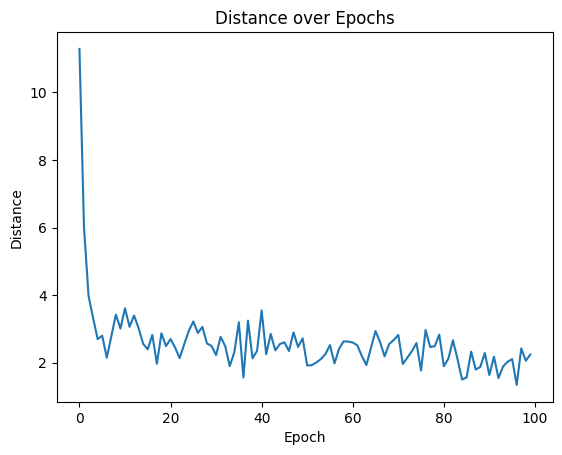
\includegraphics[width=0.8\textwidth]{Background/images/mean_std_cgan.png}
    \caption{Distance between real and generated parameters of the distribution over epochs.}
    \label{mean_std_distance}
\end{figure}


\begin{figure}[H]
    \centering
    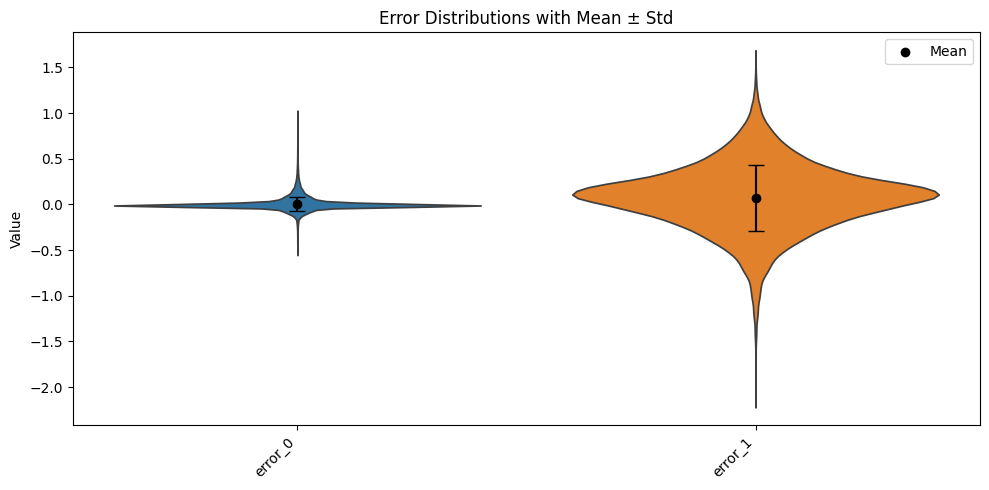
\includegraphics[width=0.9\textwidth]{Background/images/error_mean_std.png}
    \caption{Error distribution between real and generated parameters.}
    \label{mean_std_error}
\end{figure}




\section{Bins probabilities as target}
When the output representation is the bins probabilities of the normal distribution,
then logarithm transformation of the output data matrix $X$ is needed in order to avoid numerical issues and have a more stable training process.\\
In this case the distance between the real and generated distribution is measured by the Jensen-Shannon divergence
between the real and generated bins probabilities vectors.\\
However, instead of using just the Mean Absolute Percentage Error (MAPE) to run the error analysis between real and generated bins probabilities,
the Symmetric Mean Absolute Percentage Error (SMAPE) is used in order to take into account all those cases where
the real bin probability is equal to zero and that would lead to an infinite percentage error.


\subsection{Conditional GAN results}

On the first hand, a sketch of the algorithm and data flow used for training the CGAN model is shown below.
Then results obtained from training the CGAN architecture on the simulated dataset are presented.\\

\begin{algorithm}[H]
    \caption{Training process for CGAN model}
    \label{alg:cgan train}
    \begin{algorithmic}[1]

    \STATE Compute trajectories matrix $C$ and output data matrix $X$ using algorithm \ref{alg:y condition} and \ref{alg:x target}.
    \STATE Apply log transformation to data matrix $X$.
    \FOR{$i$ in $max\_epoch = 200$}
        \STATE Compute discriminator loss over true data samples $\mathcal{L}_{\text{BCE}}^{true}(1,D(x,c))
            = - \left[ 1 \log(D(x,c))\right]$ and then over generated data samples
            $\mathcal{L}_{\text{BCE}}^{fake}(0,D(G(z,c),c)) = - \left[  1\log(1 - D(G(z,c),c)) \right]$
        \STATE The Discriminator loss is then computed as $\mathcal{L}_D = \mathcal{L}_{\text{BCE}}^{true} + \mathcal{L}_{\text{BCE}}^{fake}$
        \STATE Update discriminator weights by backpropagating the loss $\mathcal{L}_D$.
        \STATE Compute generator loss over generated data samples
            $\mathcal{L}_{\text{BCE}}^{gen}(1,D(G(z,c),c)) = - \left[ 1 \log(D(G(z,c),c))\right]$   
        \STATE Update generator weights by backpropagating the loss $\mathcal{L}_G = \mathcal{L}_{\text{BCE}}^{gen}$.
    \ENDFOR
    \end{algorithmic}
\end{algorithm}

The experimental results have been obtained by training the CGAN model for 200 epochs, using the dataset and evaluation metrics described above with 
the following architecture and hyperparameters:
\begin{table}[h!]
\centering
\caption{CGAN Architecture and Hyperparameters Summary}
\label{tab:cgan_summary}
\begin{tabular}{lll}
\hline
\textbf{Parameter}         & \textbf{Generator}          & \textbf{Discriminator} \\ \hline
Input Dimension            & 252 (Latent) + 252 (Cond.)  & 100 (Data) + 252 (Cond.)         \\
Hidden Layers              & [512, 256, 256, 128]        & [512, 256, 256, 128, 64]        \\
Output Dimension           & 100                         & 1                               \\
Activation Function        & ReLU                        & Leaky ReLU                      \\
Normalization              & Batch Norm                  & None                      \\
Dropout                    & 0.0                         & 0.0                             \\
\multicolumn{3}{c}{\textbf{Global Training Settings}}                                     \\ \hline                                       \\
Generated Data Dimension (n of bins)             & \multicolumn{2}{l}{100}                             \\ \hline
Max Epochs                           & \multicolumn{2}{l}{200}                             \\ \hline
\end{tabular}
\end{table}


\begin{figure}[H]
    \centering
    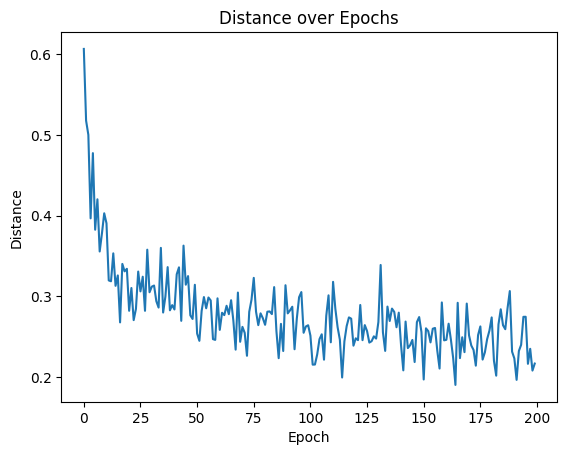
\includegraphics[width=0.9\textwidth]{Background/images/bins_global_distribution_cgan.png}
    \caption{Distance between real and generated probability density function using global bins.}
    \label{bins_global_distance}
\end{figure}

\begin{figure}[H]
    \centering
    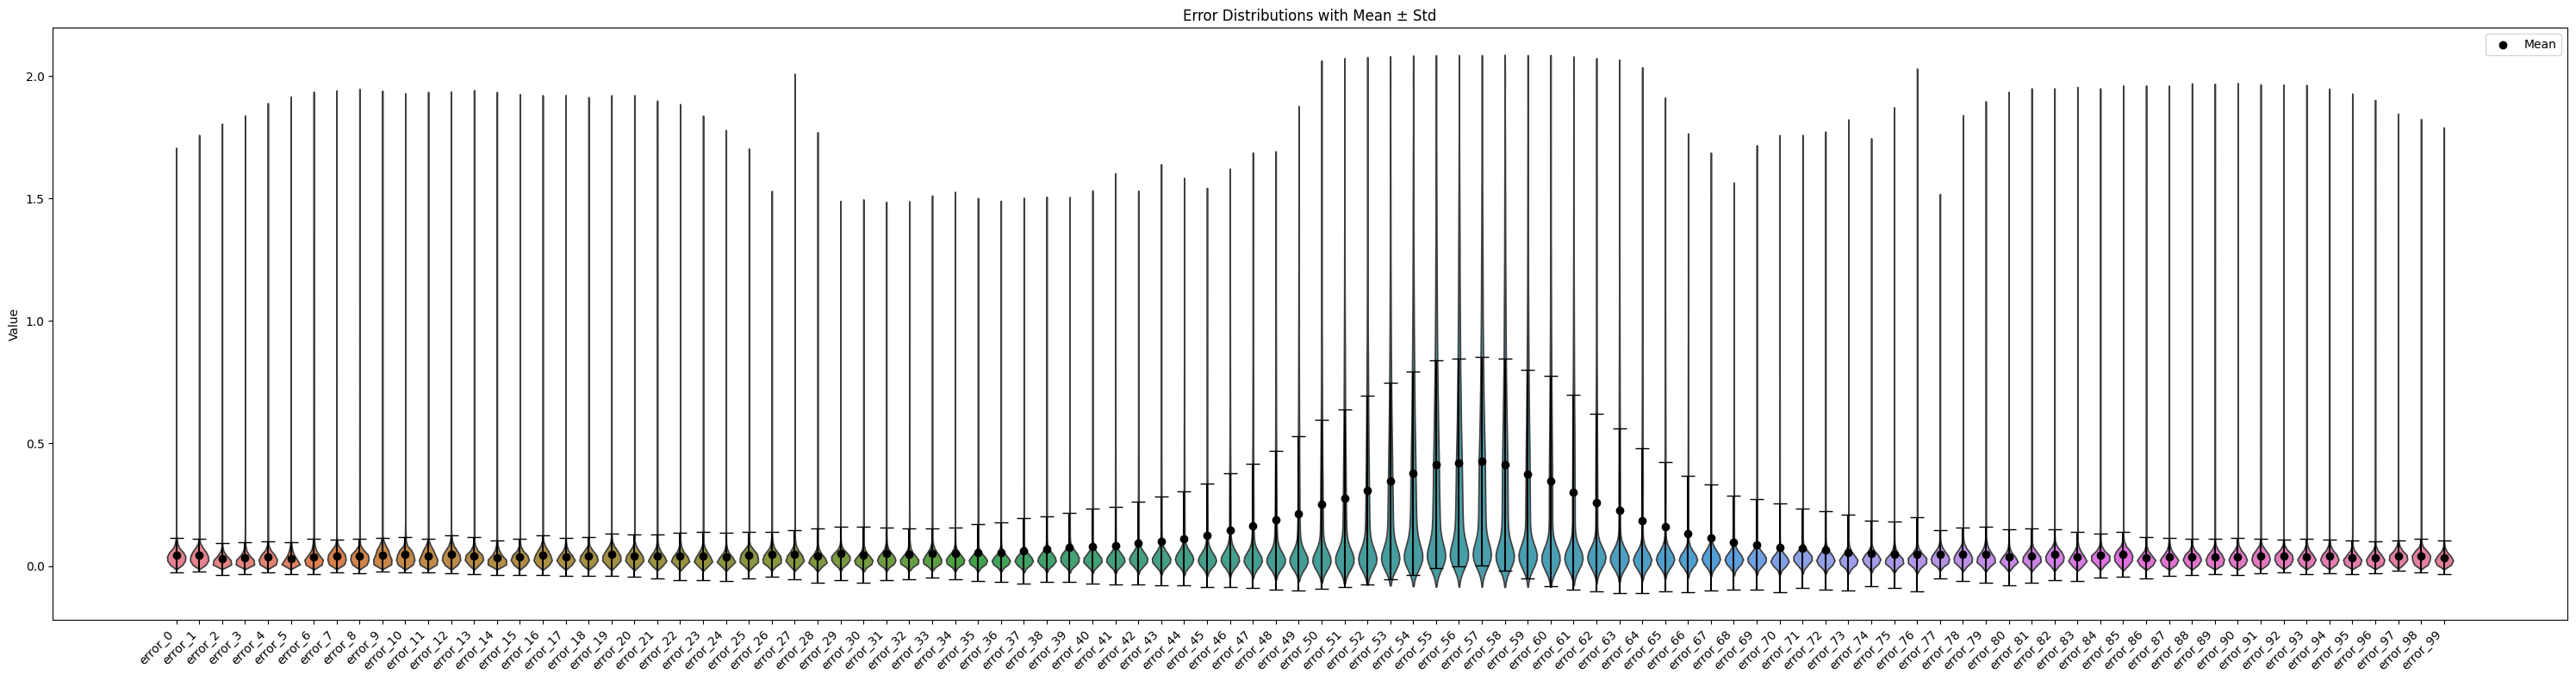
\includegraphics[width=0.9\textwidth]{Background/images/error_bins_global.png}
    \caption{Error distribution between real and generated bins probabilities using global bins.}
    \label{bins_global_error}
\end{figure}

From the results shown above in Figure \ref{bins_global_error}, it is possible to notice that tail bins have small error values since both real and generated probabilities tends to be close to zero.
Most of the errors are concentrated in central bins where the probabilities are higher and tends to be more variable. It is also important to notice the presence of error spikes,
suggesting that for some pairs of theoretical and generated distributions huge differences are present.\\
Also in this case the Kolmogorov-Smirnov test has been performed between 10000 real and generated bins probabilities, and
the resulting p-values are rejected 65\% of times, meaning that we can reject the null hypothesis
that the generated distribution are equivalent to the theoretical ones in 65 percent of the cases.\\

\begin{table}[h]
\centering
\begin{tabular}{l c}
\hline
\textbf{Metric} & \textbf{Value} \\
\hline
KS-Test acceptance rate & 0.35 \\
JS Distance & 0.3430 \\
Hellinger Distance & 0.3067 \\
TV Distance & 0.3078 \\
\hline
\end{tabular}
\caption{CGAN performance metrics averaged over 10000 samples}
\end{table}


In order to test the generalization capabilities of the model,
different samples have been drawn such that every sampling parameter is fixed except for the volatility $\sigma$.
In particular, six different samples are shown below where
the starting values is the same $X_0 = 0.0$, $\mu = 0.0$ while the volatility have different values for each sample 
$\sigma = [0.1, 0.3, 0.5, 0.7, 0.9, 0.11]$. 
\begin{figure}[H]
    \centering
    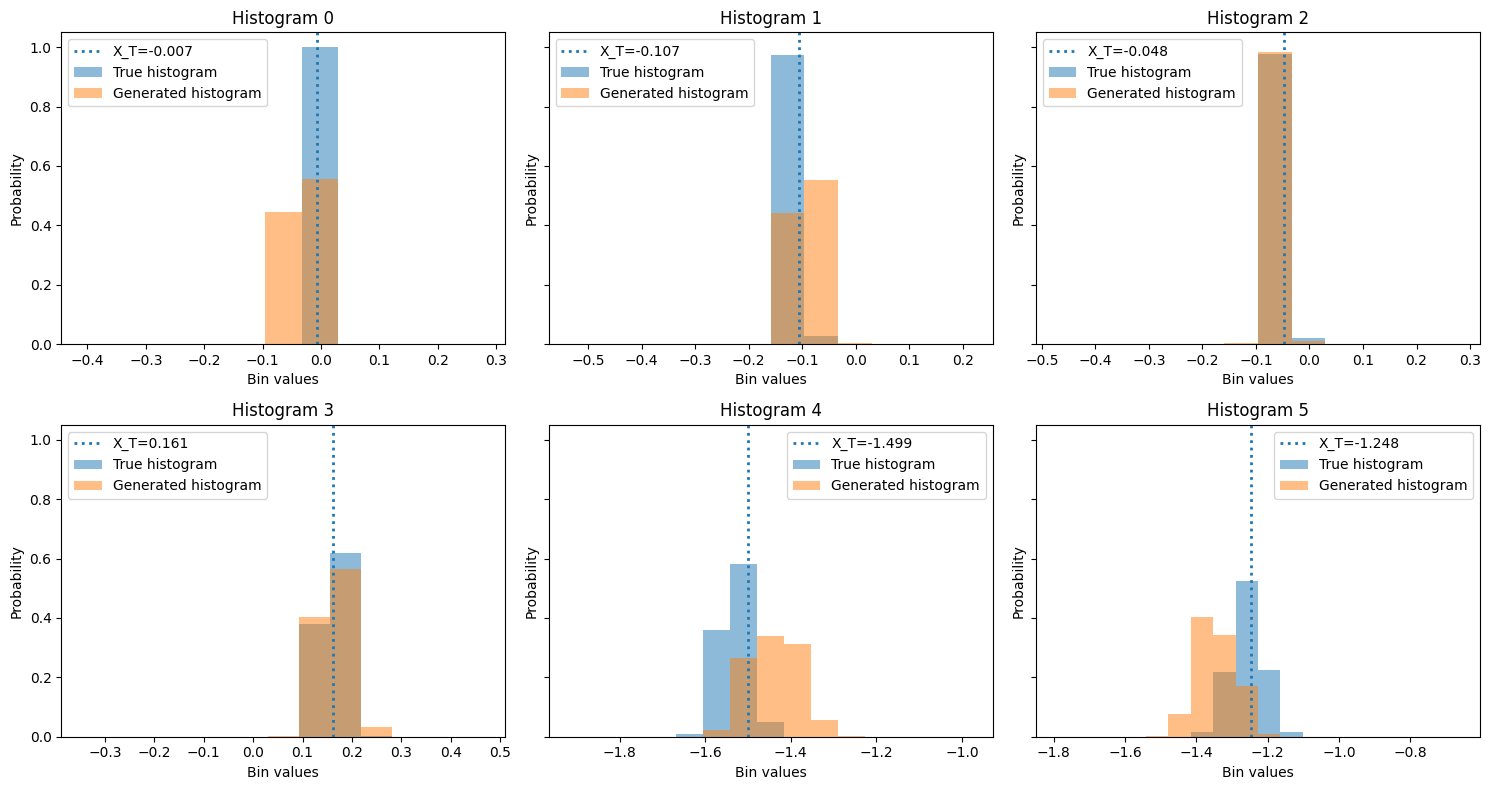
\includegraphics[width=1.0\textwidth]{Background/images/bins_samples_sigma.png}
    \caption{Samples obtained using fixed $X_0$ and $\mu$ while varying $\sigma = [0.1, 0.3, 0.5, 0.7, 0.9, 0.11]$.}
    \label{bins_global_sample_sigma}
\end{figure}

From the results shown above, it is possible to observe that the model is able to
effectively capture the first moment of the distribution since it is usually alligned with the theoretical distribution.
However, it struggles to accurately model the second moment, especially when the volatility is high.
This would lead to underestimate or overestimate tail risk in financial applications.

\subsection{Conditional Wasserstein GAN results}
In this section, we present the results obtained from training the CWGAN architecture on the same dataset used for the CGAN experiments, 
by following the same data simulation, preprocessing, and evaluation procedures described before.\\


\begin{algorithm}[H]
    \caption{Training process for CWGAN-GP model}
    \label{alg:cwgan train}
    \begin{algorithmic}[1]

    \STATE Compute trajectories matrix $C$ and output data matrix $X$ using algorithm \ref{alg:y condition} and \ref{alg:x target}.
    \STATE Apply log transformation to data matrix $X$.
    \FOR{$i$ in $max\_epoch = 100$}
        \STATE Compute the critic real value output for true data samples $D(x,c)$ and then for generated data samples $D(G(z,c),c)$.
        \STATE Compute the gradient penalty term $GP$ as defined in \ref{alg:gradient_penalty}.
        \STATE Compute critic loss $\mathcal{L}_D$ following \ref{alg:cwgan_gp} with the addition of the gradient penalty term.
        \STATE Update critic weights by backpropagating the loss $\mathcal{L}_D$.
        \STATE Compute generator loss $\mathcal{L}_G$ following \ref{alg:cwgan_gp}.
        \STATE Update generator weights by backpropagating the loss $\mathcal{L}_G$.
    \ENDFOR
    \end{algorithmic}
\end{algorithm}

The experimental results have been obtained by training the CWGAN-GP model for 100 epochs, using the same dataset and evaluation metrics as in the CGAN case with 
the following architecture and hyperparameters:
\begin{table}[h!]
\centering
\caption{CWGAN Architecture and Hyperparameters Summary}
\label{tab:cwgan_summary}
\begin{tabular}{lll}
\hline
\textbf{Parameter}         & \textbf{Generator}          & \textbf{Critic (Discriminator)} \\ \hline
Input Dimension            & 252 (Latent) + 252 (Cond.)  & 100 (Data) + 252 (Cond.)         \\
Hidden Layers              & [512, 256, 256, 128]        & [512, 256, 256, 128, 64]        \\
Output Dimension           & 100                         & 1                               \\
Activation Function        & ReLU                        & Leaky ReLU                      \\
Normalization              & None                        & Layer Norm                      \\
Dropout                    & 0.0                         & 0.0                             \\
\multicolumn{3}{c}{\textbf{Global Training Settings}}                                     \\ \hline                                       \\
Generated Data Dimension (n of bins)           & \multicolumn{2}{l}{100}                          \\ \hline   
Max Epochs                           & \multicolumn{2}{l}{100}                                       \\ \hline
\end{tabular}
\end{table}

\begin{figure}[H]
    \centering
    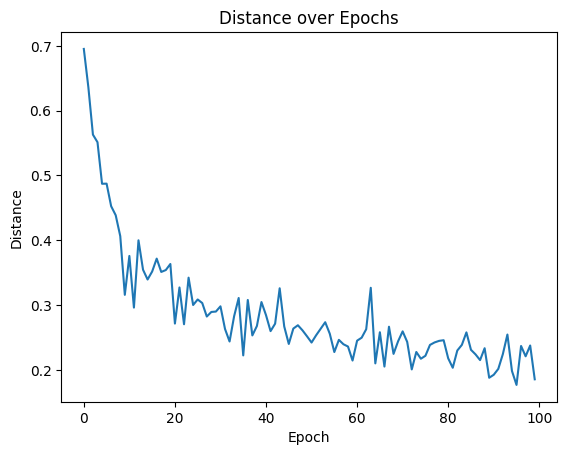
\includegraphics[width=0.9\textwidth]{Background/images/bins_global_distribution_cwgan.png}
    \caption{Distance between real and generated probability density function of the standard normal distribution over epochs.}
    \label{cwgan_curve}
\end{figure}



\begin{figure}[H]
    \centering
    \includegraphics[width=1.0\textwidth]{Background/images/CWGAN_error_dist.png}
    \caption{Error distribution between real and generated bins probabilities using global bins.}
    \label{cwgan_global_error}
\end{figure}



\begin{figure}[H]
    \centering
    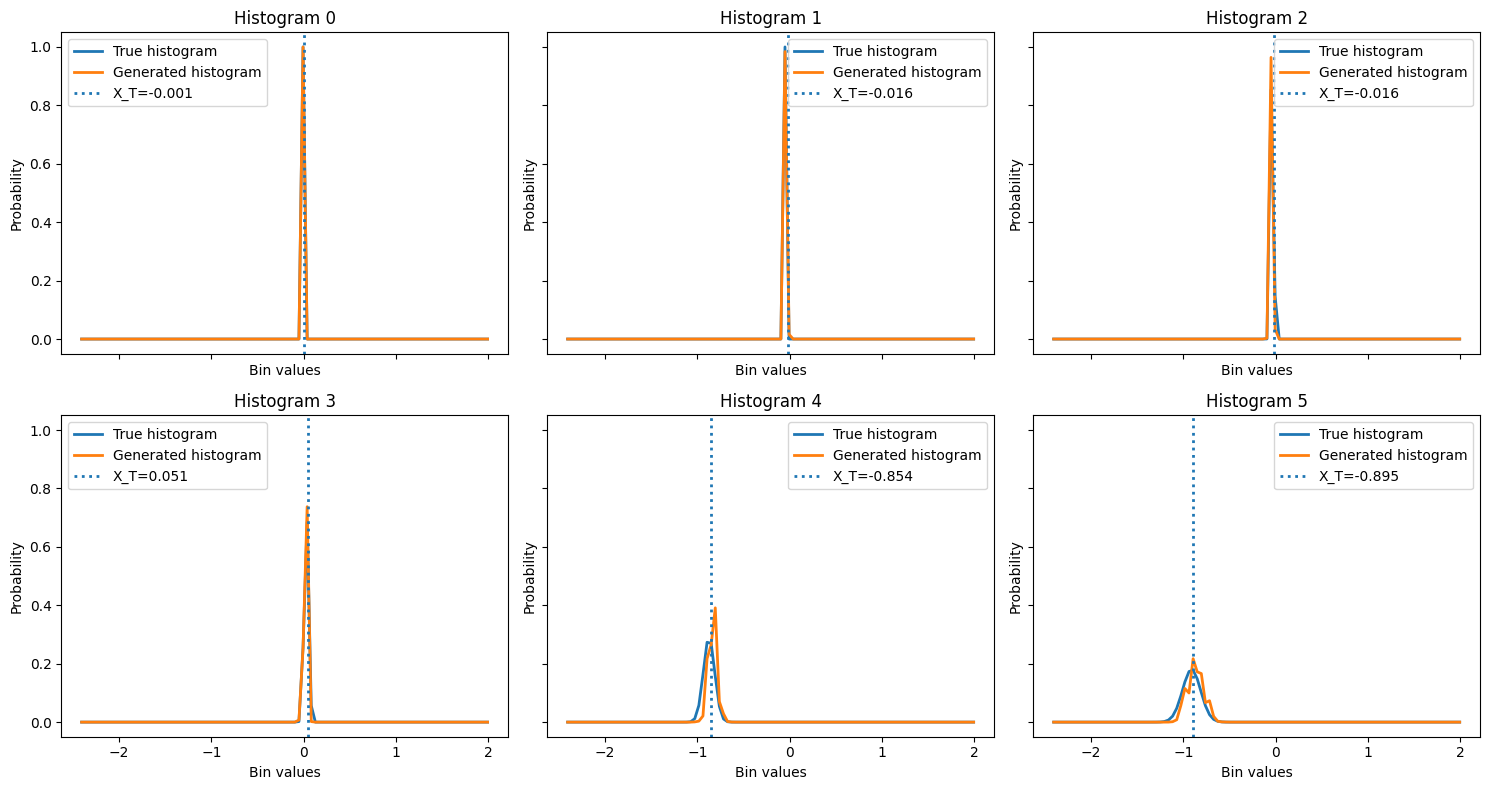
\includegraphics[width=1.0\textwidth]{Background/images/cwgan_samples_sigma.png}
    \caption{Samples obtained using fixed $X_0$ and $\mu$ while varying $\sigma = [0.1, 0.3, 0.5, 0.7, 0.9, 0.11]$.}
    \label{cwgan_sample_sigma}
\end{figure}


As can be seen from \ref{cwgan_sample_sigma} the quality of the generated distributions is significantly improved with respect to the CGAN results shown in \ref{bins_global_sample_sigma}.
This is also confirmed by running the Kolmogorov-Smirnov test over 10000 generated samples. The results show that
53\% of the generated samples are accepted at a significance level of 1\%, compared to only 35\% acceptance rate for the CGAN model.\\

\begin{table}[h]
\centering
\begin{tabular}{l c}
\hline
\textbf{Metric} & \textbf{Value} \\
\hline
KS-Test acceptance rate & 0.53 \\
JS Distance & 0.3050 \\
Hellinger Distance & 0.2712 \\
TV Distance & 0.2725 \\
\hline
\end{tabular}
\caption{CWGAN-GP performance metrics averaged over 10000 samples}
\end{table}

However, the model still provide poor performances since for higher values of $\sigma$ the generated distributions tends to be rejected from the KS test, suggesting lack of capacity to model the full range of the target distribution for trajectories with high volatility.
Moreover, the average Jenshen-Shannon divergence between real and generated distributions over the 10000 samples is around 0.20 which is not an excellent result considering that the JS-divergence is bounded between 0 and 1.
These poor performances arises from the main drawback of the proposed architecture, which is the discretization of the output distribution into a fixed number of bins. 
This approach can lead to loss of information and may not capture the full complexity of the underlying distribution, especially in cases where the chosen number of bins is insufficient to represent the true distribution, particularly if the distribution has heavy tails or is multimodal.

\section{Possible improvements}
The main issue that need to be addressed in order to produce coherent distributions is to produce a meaningful representation of the output to be generated 
in order to effectively capture the variance of the target distribution, 
avoiding in this way underestimation or overestimation of extreme events.
Different approaches have been adopted in the literature to adapt the GAN architecture to time series data, with the aim
of improving training stability, convergence of GANs and solve the mode collapse problem.\\

Specific techniques can be employed to better capture the distributional characteristics of financial time series data.
Some of these techniques are discussed in academic papers like \cite{background:forgan}, \cite{background:md_cgan} and \cite{background:rcgan}:
\begin{itemize}
    \item For example, in \cite{background:rcgan} both the generator and discriminator are RNN or LSTM networks adopted to better capture the sequential dependencies in time series data.
    \item Predict the values corresponding to a fixed set of quantiles. 
    The model generates the outcome values associated with specified probability levels for example $[0.01, 0.1, 0.25, 0.5, 0.75, 0.9, 0.99]$.
    Usually this approach is used in quantile regression where the loss function is the quantile loss, which is specifically designed to provide consistent estimation of conditional quantiles.
    \item Model the output distribution as a mixture of Gaussians, where the generator predicts the parameters of the mixture components (means, variances, and mixing coefficients) as proposed in \cite{background:md_cgan}.
    \item The generated output can be the value of the time step for which we would like to generate the distribution. So after training,
    at inference time, the distribution can be recovered by repeatedly evaluating the generator for a fixed input trajectory while varying the random noise.
    The collection of generated outputs, for example 1000 samples, constitutes an empirical approximation of the conditional predictive distribution as discussed in \cite{background:forgan}.
    \item Adding a term to the generator's loss that penalizes it if the mean and variance of a batch of generated samples don't match the mean and variance of the "real" theoretical samples.
\end{itemize}

However, in this work, the focus is on the architecture proposed in \cite{background:forgan} possibly with some improvements in order to generate a more meaningful representation of the output distribution, for 
financial processes characterized by high volatility and heavy tails. The proposed architecture is discussed in the next chapter.

%\chapter{Conditional Wasserstein GAN}

In this chapter, we introduce the Conditional Wasserstein Generative Adversarial Network (CWGAN) architecture,
which extends the traditional conditional GAN framework by means of the Wasserstein distance exploitation.\\

The main changes that characterize the CWGAN with respect to the CGAN are:
\begin{itemize}
    \item The loss function of a standard GAN is based on Jensen-Shannon divergence minimization while the CWGAN is based on the Wasserstein distance, which provides a more stable training process and mitigates issues such as mode collapse.
    \item The discriminator, which in Wasserstein GAN architecture is called critic, is designed to output real-valued scores instead of probabilities, allowing it to better capture the differences between real and generated data distributions.
    For this reason, the discriminator network does not use a sigmoid activation function in the output layer.
    \item The training procedure requires as a good practice to optimize the critic multiple times per generator update to ensure that the critic provides accurate gradients for the generator.
    \item The use of gradient penalty term in the loss function has the objective to enforce the Lipschitz constraint required for the Wasserstein distance computation.  
\end{itemize}


Now the critic maximizes the following loss function $E_{\boldsymbol{x} \sim p_d}[D(\boldsymbol{x})]-E_{\widehat{\boldsymbol{x}} \sim p_g}[D(\widehat{\boldsymbol{x}})]$ where $\boldsymbol{x}$ are real data samples from the data distribution $p_d$ and $\widehat{\boldsymbol{x}}$ are generated samples from the generator distribution $p_g$.
On the other hand, the generator minimizes the loss function $-E_{\widehat{\boldsymbol{x}} \sim p_g}[D(\widehat{\boldsymbol{x}})]$.\\
Given this setup, there is no need anymore for true and fake data labels since the critic outputs real-valued scores.\\
An additional advatage of using the Wasserstein distance is that it provides a meaningful measure of the distance between the real and generated data distributions, which allows for the implementation of an early stopping technique which
improve the training efficiency.\\

\section{Experiment results}
In this section, we present the results obtained from training the CWGAN architecture on the same dataset used for the CGAN experiments, 
by following the same data simulation, preprocessing, and evaluation procedures described before.\\



\begin{figure}[H]
    \centering
    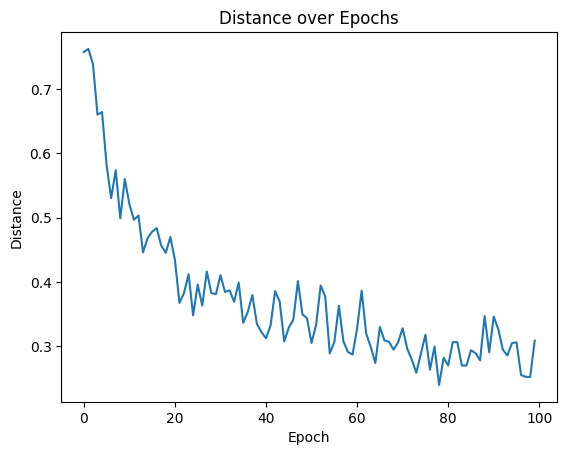
\includegraphics[width=0.9\textwidth]{Background2/images/CWGAN_learning_curve.png}
    \caption{Distance between real and generated probability density function of the standard normal distribution over epochs.}
    \label{cwgan_global_error}
\end{figure}



\begin{figure}[H]
    \centering
    \includegraphics[width=1.0\textwidth]{Background2/images/CWGAN_error_dist.png}
    \caption{Error distribution between real and generated bins probabilities using global bins.}
    \label{cwgan_global_error}
\end{figure}



\begin{figure}[H]
    \centering
    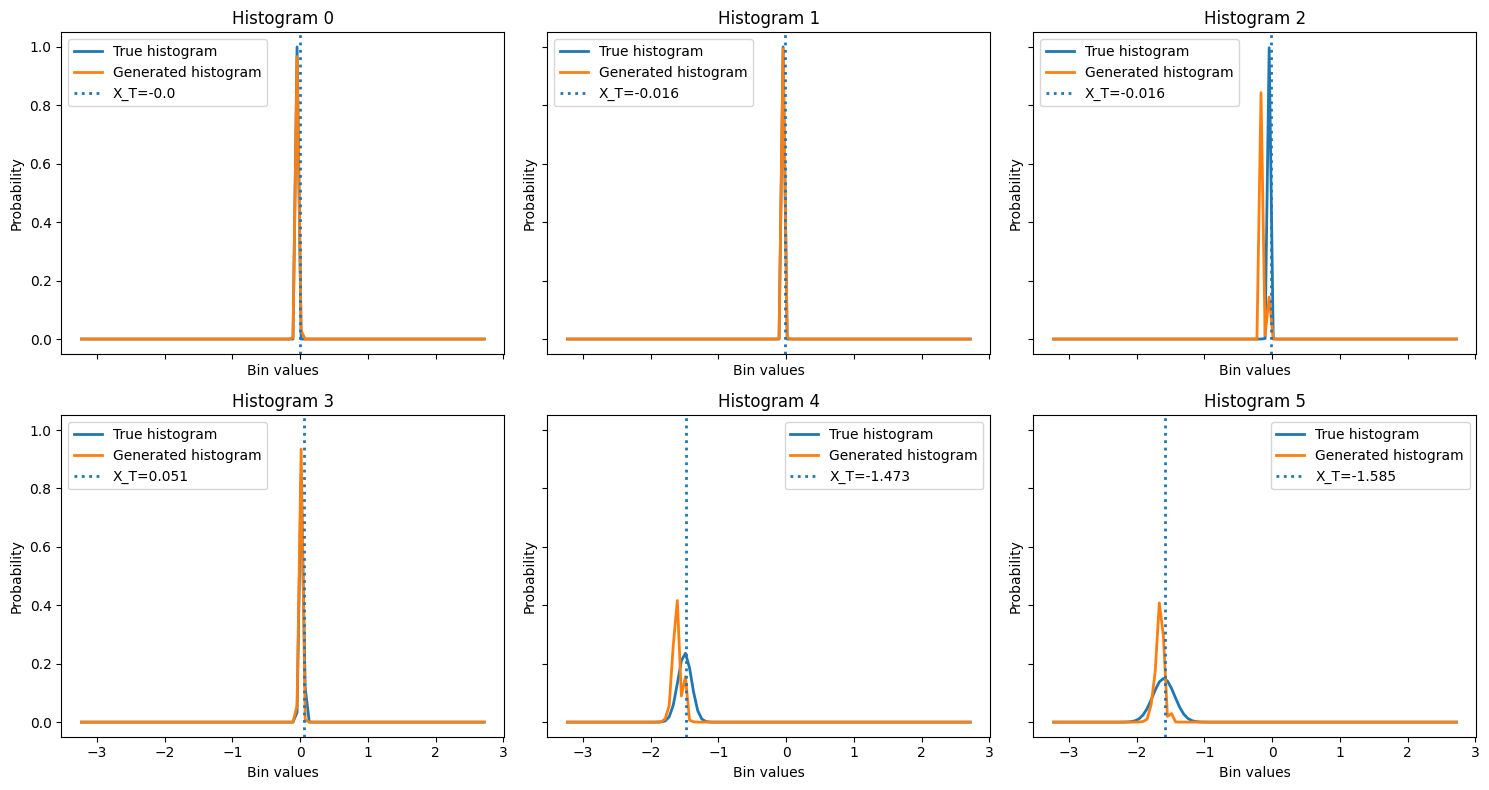
\includegraphics[width=1.0\textwidth]{Background2/images/CWGAN_bins_samples_v2.png}
    \caption{Samples obtained using fixed $X_0$ and $\mu$ while varying $\sigma = [0.001, 0.01, 0.05, 0.1, 0.5, 0.8]$.}
    \label{cwgan_sample_sigma}
\end{figure}


As can be seen from \ref{cwgan_sample_sigma} the quality of the generated distributions is significantly improved with respect to the CGAN results shown in \ref{bins_global_sample_sigma}.
This is also confirmed by running the Kolmogorov-Smirnov test over 1000 generated samples. The results show that
30\% of the generated samples are accepted at a significance level of 1\%, compared to only 2.5\% acceptance rate for the CGAN model.\\
However, the model is still not perfect since for higher values of $\sigma$ the generated distributions still deviate from the real ones.
Further hyperparameter tuning and model architecture adjustments may be necessary to achieve better performance.





%\nocite{*}
\printbibliography

\end{document}